\chapter{支持QoS关联的组合服务Skyline计算}

\section{引言}

Web服务是一个平台独立的,低耦合的,自包含的、基于可编程的web的应用程序,可使用开放的XML (标准通用标记语言下的一个子集)标准来描述、发布、发现、协调和配置这些应用程序,用于开发分布式的互操作的应用程序。在面向服务的体系架构中,服务提供者将其业务包装为服务并对外发布,服务消费者根据自身业务需要,查找满足自身需求的服务进行调用。随着面向服务计算的技术被广泛的应用,提供类似或者相同功能的Web服务越来越多,服务质量逐渐成为不同服务提供商之间竞争的主要因素,同时也是消费者关注的重点。在一些面向服务的应用中,服务集成商依据用户的功能性需求,以及非功能性的QoS约束,在已有的备选服务中进行挑选,并对选中的备选服务进行组合,从而为消费者提供功能更为强大的组合服务。但是如何高效的为消费者选择出既可满足其功能的需求又可提供最高的服务质量组合服务,是服务集成商特别关注的问题。通常,在选择的过程中,简单加权技术(Simple Additive Weighting,~SAW)被广泛的应用。

然而在实际的应用场景中,这些方法仍有一些缺点:
(1)消费者需要在自己关注的多个服务质量属性之间进行权衡,并将这种权衡转为具体的数字作为权重提供给服务集成商,但这种方式对于消费者来说无疑是很有挑战的一件事情,因为有的时候消费者自己也不能准确的描述每一个属性对自己的重要程度,因此当服务集成商给消费者返回结果后,消费者也许并不满意,进而会重新指定新的权重给服务集成商,在服务集成商接到新的请求后,需要重新进行计算。除此之外,如果这种请求很频繁的话,会导致服务集成商端产生大量的计算~\cite{yu2013efficient}~;
(2)对于发起相同功能请求的不同消费者,他们对服务质量属性所指定权重很有可能是不同的,因而为了满足这些消费者,服务集成商需要重复在候选服务集合中挑选,并组合出满足这些消费者需求的不同组合服务,但当候选服务集合中服务备选服务的数量较大时,这些请求会导致服务集成商端产生了大量的计算。
为了提高服务集成商服务选择效率,一些学者利用了Skyline技术中的支配关系,在每一个候选服务集合中选择一组Skyline服务,移除了一些不可能出现在~QoS~ 最优组合服务中的服务,从而到达减少候选服务搜索空间提高服务选择效率的目的。虽然利用这种方法可以在一定程度上提高了服务选择的效率,但是当面对上述情况上,仍需要每次都遍历所有的候选服务集合,进行服务选择,不同只是候选服务集合的大小变化了。为了解决上述问题,Yu Qi~\cite{yu2013efficient}~提出了组合服务Skyline的概念,利用支配关系在所有的组合服务中选择出一组`` 最好''的组合服务,这些服务构成了组合服务Skyline。 利用组合服务Skyline,服务集成商在面对上述问题时候,不需要每次通过重新搜索候选服务集合计算QoS最优组合服务,而是在组合服务Skyline 中去搜索即可。

我们再来看一个\emph{旅行准备}例子,消费者希望做好旅行的准备工作,服务集成商为消费者提供了一个方案(图~\ref{F:Fig_CorrExmp}~ 中上半部分的抽象组合服务),每一个步骤(抽象组合服务中的抽象服务)中都对应着许多实现方式(图~\ref{F:Fig_CorrExmp}~ 中下半部分的原子服务)。如果我们在线旅游服务选择的是\emph{阿里去啊}$\footnote{\url{http://www.alitrip.com/}}$,并且航班服务选择\emph{南方航空}$\footnote{\url{http://www.csair.com/}}$,那么\emph{南方航空}的机票的售价就会降低,如图~\ref{F:Fig_CorrExmpAli}~ 所示。除此之外,我们知道服务在被调用时通常需要先对身份进行验证(如:检查是否登录),然后才可以对服务进行调用。因此,如果我们在线旅游服务选择的是\emph{阿里去啊},并且购买旅行用品的时候,我们选择的是\emph{淘宝}$\footnote{\url{http://www.taobao.com/}}$,由于它们都是由阿里巴巴集团提供,账户通用,因此我们在调用\emph{淘宝}的时候,就省去了身份验证的步骤,从而降低了该服务的响应时间。

\begin{figure}[thb]
    \centering
    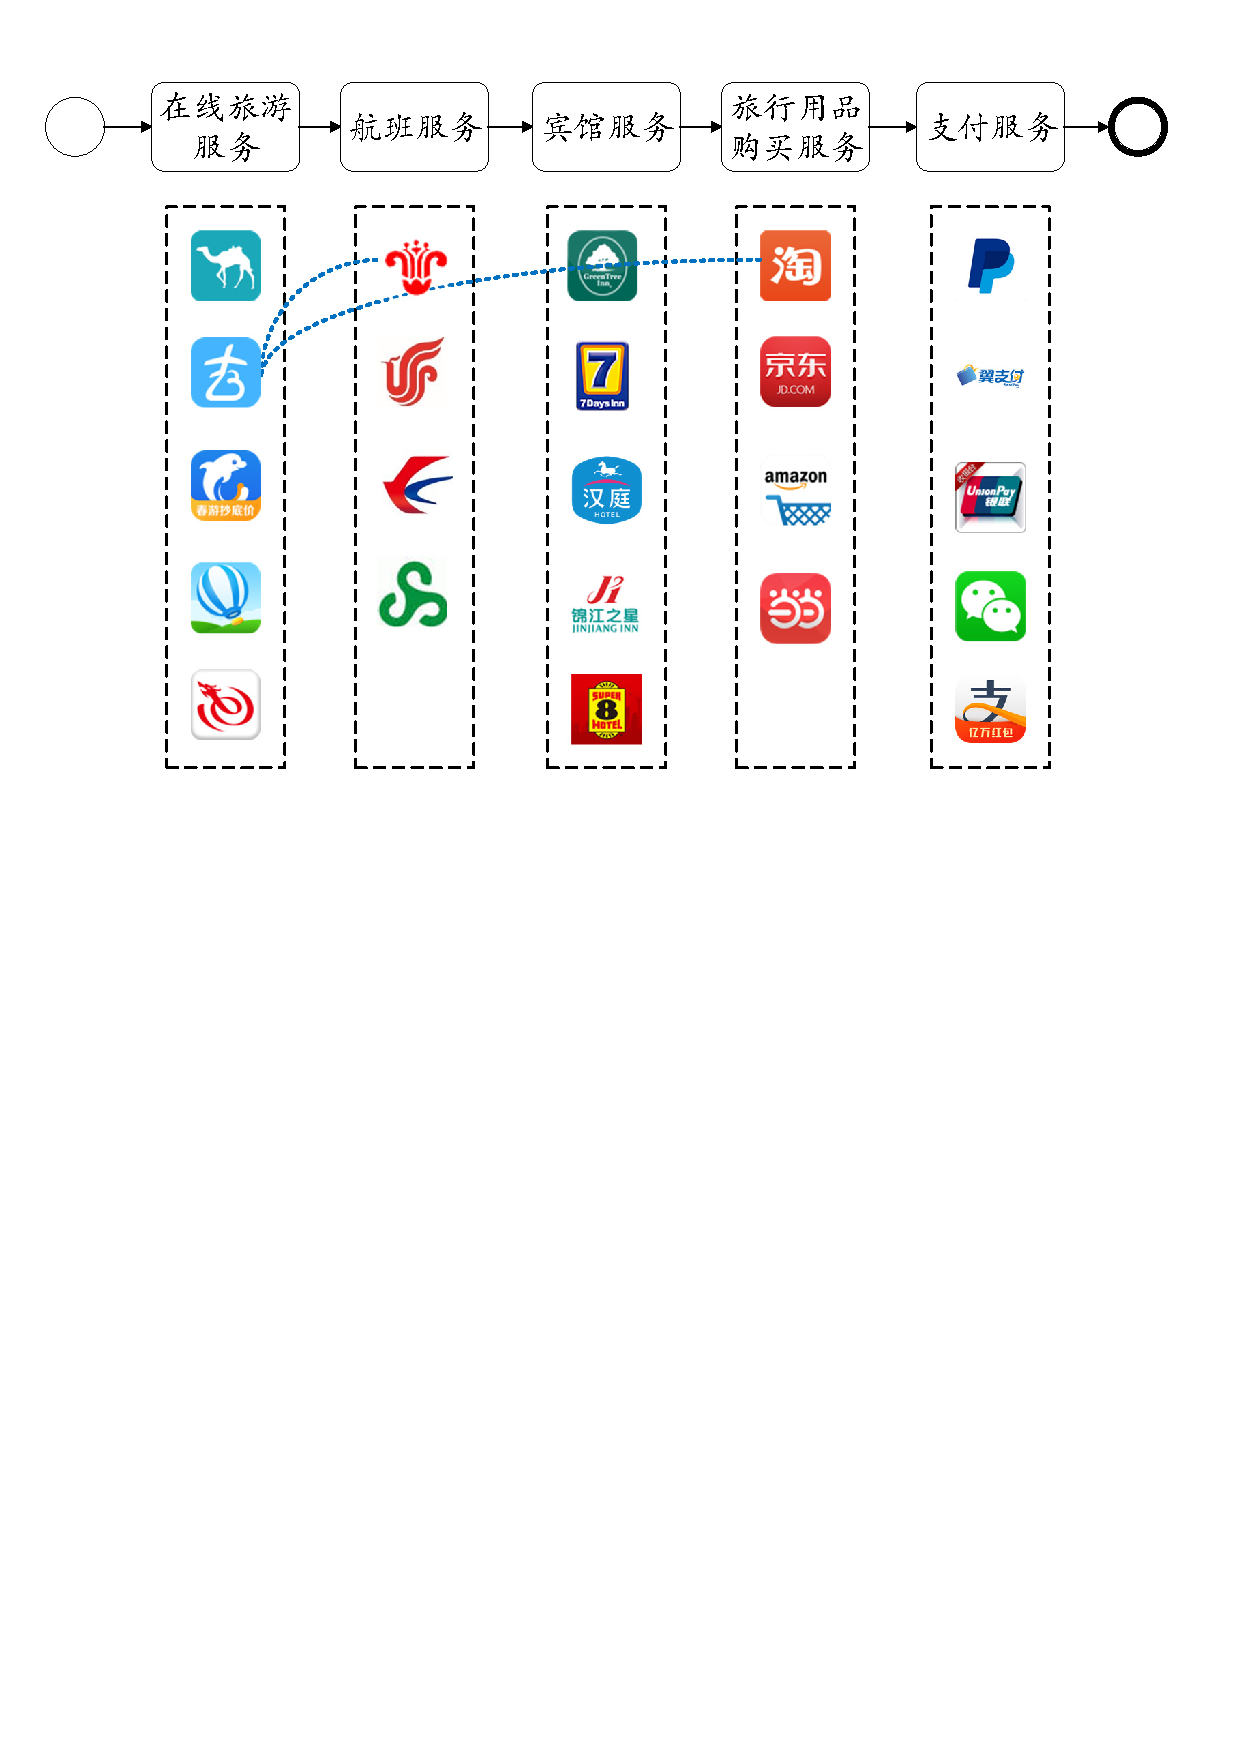
\includegraphics[width=0.8\textwidth]{./FIGs/Fig_CorrExmp.pdf}
    \caption{服务组合:旅行准备}
    \label{F:Fig_CorrExmp}
\end{figure}

\begin{figure}[thb]
    \centering
    
\includegraphics[width=0.8\textwidth]{./FIGs/Fig_CorrExmpAli.png}
    \caption{QoS关联的例子:价格}
    \label{F:Fig_CorrExmpAli}
\end{figure}

这些例子都说明了服务与服务之间不是独立的,一个可选服务的服务质量很有可能依赖于其他的可选服务,上述提到的工作由于缺乏对这种关联关系的考虑,使得最终选出的组合服务的QoS实际上并不是最优的,从而无法在最大程度上满足消费者的需求。

我们希望在考虑QoS关联的情况下,计算出组合服务Skyline。最简单的方法是遍历所有可能的组合服务,利用Skyline中的支配关系选择出组合服务Skyline。然而这种方法仅适用于每一个抽象服务所对应的候选服务集合中服务数量较小的情况。当候选服务集合的服务数量比较大时,会导致组合爆炸的问题,致使计算组合服务Skyline的效率非常低下。虽然利用Yu Qi在文献~\cite{yu2013efficient}~中提出的方法可以提高计算的效率,但是由于他没有将QoS关联关系考虑到计算之中,导致按照他的方法来计算组合服务Skyline 的结果并不准确。

为了解决这个问题,我们提出了一种支持QoS关联关系的组合服务Skyline计算方法,以及两个剪枝算法,用来在计算组合服务Skyline 前,移除候选服务集合中的冗余服务。我们不可以单纯的利用支配关系来移除冗余服务,这样做会导致我们在移除具有QoS关联关系服务的时候产生错误。在本章接下来的内容中,将对上述提到的方法进行详细的介绍。

\section{背景}

在本节,我们将会对我们的研究动机进行说明,然后给出支持QoS关联的服务模型,最后给出我们的问题定义。

\subsection{研究动机}\label{S:SEC_Motivation}

为了解释我们的研究动机,我们将在本节给出一个具体的例子。在表~\ref{T:Tab_WSSet}~ 中,展示了三个抽象服务,每一个抽象服对应着四个原子服务(在同一个候选服务集合中),为了简单起见,在这个例子中,我们仅考虑两个QoS属性,\emph{价格}和\emph{响应时间},并且假设QoS关联关系只存在于\emph{价格}属性上。服务之间的QoS 关联关系我们用``select()'' 来表示,比如,$z_{4}$所在单元格中的select($y_{4}$) 就表示:如果我们在一个组合服务中同时选择了$y_{4}$ 以及$z_{4}$,$z_{4}$的价格就降低为\$5。QoS\emph{关联值}我们用深蓝色且带下划线的字体呈现。对于每个候选服务集合中的Skyline 服务我们用红色加粗的字体表示。

%表格:服务集合
\begin{table}[tp]
\centering  % 表居中
\begin{tabular}{|c|c|c|}  % {} 表示各列元素对齐方式,left-l,right-r,center-c
\hline
\emph{X} & \emph{Y} & \emph{Z}\\ \hline\hline
%第1行
\emph{x}$_{1}$: (\$10, 0.7s)
&\textcolor[rgb]{1.00,0.00,0.00}{\textbf{\emph{y}$_{1}$}}: (\$12, 0.4s)
&\tabincell{c}{\emph{z}$_{1}$: (\$7, 1.0s)\\ %dark blue
select(\emph{x}$_{1}$): (\textcolor[rgb]{0.0, 0.0, 0.55}{\underline{\$6}}, 1.0s)\\
select(\emph{y}$_{1}$): (\textcolor[rgb]{0.0, 0.0, 0.55}{\underline{\$5}}, 1.0s)}
\\ \hline
%第2行
\emph{x}$_{2}$: (\$4, 0.5s)
&\emph{y}$_{2}$: (\$15, 0.5s)
&\tabincell{c}{\emph{z}$_{2}$: (\$8, 0.7s)\\
select(\emph{y}$_{1}$): (\textcolor[rgb]{0.0, 0.0, 0.55}{\underline{\$5}}, 0.7s)}
\\ \hline
%第3行
\emph{x}$_{3}$: (\$5, 0.3s)
&\tabincell{c}{\textcolor[rgb]{1.00,0.00,0.00}{\textbf{\emph{y}$_{3}$}}: (\$12, 0.4s)\\ %dark blue
select(\emph{x}$_{2}$): (\textcolor[rgb]{0.0, 0.0, 0.55}{\underline{\$11}}, 0.4s)\\
select(\emph{x}$_{3}$): (\textcolor[rgb]{0.0, 0.0, 0.55}{\underline{\$10}}, 0.4s)}
&\textcolor[rgb]{1.00,0.00,0.00}{\textbf{\emph{z}$_{3}$}}: (\$6, 0.7s)
\\ \hline
%第4行
\textcolor[rgb]{1.00,0.00,0.00}{\textbf{\emph{x}$_{4}$}}: (\$4, 0.3s)
&\emph{y}$_{4}$: (\$17, 0.6s)
&\tabincell{c}{\emph{z}$_{4}$: (\$10, 0.9s)\\ %dark blue
select(\emph{y}$_{4}$): (\textcolor[rgb]{0.0, 0.0, 0.55}{\underline{\$5}}, 0.9s)}
\\ \hline
\end{tabular}
\caption{候选服务集合}\label{T:Tab_WSSet}
\end{table}
%表格结束:服务集合

给定一组Web服务,一个服务支配另一个服务,当且仅当该服务的每一个属性都优于或者等于另一个服务的相应属性,且至少有一个属性是完全优于另一个服务的相应属性。对于这一组Web服务来说,Skyline计算是指从所有服务中选出一组不被任何其他服务支配的服务集合。组合服务Skyline与Skyline服务类似,它是指从一组候选组合服务中,选出不被其他组合服务支配的组合服务集合。

\begin{example}[组合服务Skyline]\label{EX:Examp_CSKY}

假设我们需要利用表\emph{~\ref{T:Tab_WSSet}~}中的三个抽象组合服务按照顺序结构将它们集成,构造出一个抽象组合服务,这个抽象组合服务一共有$4^{3}=64$ 种可能组合服务,在这些组合服务中可以计算得出组合服务Skyline 为$\{\{x_{3},y_{3},z_{3}\},\{x_{4},y_{1},z_{2}\}\}$。
\end{example}

如果直接应用文献~\cite{yu2013efficient}~中提出的BUA算法,我们得到的组合服务Skyline将是$\{\{x_{4},y_{1},z_{3}\},\{x_{4},y_{3},z_{3}\}\}$,该结果与实际的结果完全不同。之所以会产生这样的错误,是因为在BUA 算法中并没有考虑QoS关联对服务的QoS值产生的影响。BUA 算法采取的是混合策略,简单来说,它先用一个局部搜索策略,在每一个候选服务集合中选出服务Skyline,然后基于这些Skyline服务计算出组合服务Skyline。从而对于不属于Skyline 的服务,将会被直接被丢弃。然而在具有QoS 关联的应用场景中,这么做显然存在一个明显的缺点:有一些服务(比如:$s$)虽然不是Skyline 服务,但是服务$s$ 与其他服务存在着QoS 关联,当$s$与这些服务组合的时候,会使得含有$s$ 的组合服务的QoS 属性值变得更好,从而这个组合服务有可能出现在最后的组合服务Skyline 中。

除此之外,虽然采取穷举的方法可以计算出正确的组合服务Skyline,但是在候选服务集合中服务数量很大的时候,采取这种做法会产生组合爆炸的问题。

由于以上这些原因的存在,我们希望提出一种方法,使其在存在QoS 关联的场景下,依然可以高效且准确的计算出组合服务Skyline。

%那么有一些服务,虽然不是Skyline服务,但是其与某一些服务的关联QoS值可能非常低,从而使得其
%
%虽然BUA算法不能直接用于考虑QoS关联的场景中,但是其局部策略仍然给我们一些启发:尽可能多的删除无用的服务。

\subsection{支持QoS关联的服务建模}\label{S:SEC_CorrModel}

\begin{definition}[抽象组合服务]

抽象组合服务$\emph{ACS}=\{S_{1}, S_{2}, \cdots, S_{m}\}$,\emph{ACS}包含了$m$个抽象服务。每一个抽象服务$S_{i}$都有一个候选服务集合与之对应,$\emph{CndS}_{i}=\{s_{i1}, s_{i2}, \cdots, s_{in}\}$。

\end{definition}

\begin{definition}[组合服务]

组合服务是在每一个候选服务集合中选择一个候选服务与抽象组合服务中的抽象服务绑定,所形成的增值服务,$\emph{CS}=\{s_{1i_{1}}, s_{2i_{2}}, \cdots, s_{mi_{m}}\}$。

\end{definition}


\begin{definition}[服务质量]

服务$s$的服务质量$\emph{Q}(s)=\{q_{1}, q_{2}, \cdots, q_{d}\}$,表示服务$s$ 有$d$ 个\emph{QoS} 属性。$s$的\emph{QoS}值为$\emph{QV}(s)=\{q_{1}(s), q_{2}(s), \cdots, q_{d}(s)\}$,其中$q_{i}(s)$为$s$ 的第$i$个质量属性的属性值。

\end{definition}

QoS属性一般分为两类:一类是\emph{正属性},通常服务质量属性越好,其属性值越高,例如:可靠性;另一类是\emph{负属性},通常服务质量属性越好,其属性值越低,例如:价格。

%\textcolor[rgb]{1.00,0.00,0.00}{\textbf{记得加$\sim$ 号!!!!!!!!!!!!!!!!!!!!!!!!!!!!!!!!!!!!!!!!!!!!!!!!!!!!!!!!!!!!!!!!!!!!}}

\begin{definition}[QoS关联]

一个服务~$a$~的~\emph{QoS}~关联~$c=<q,\ cv,\ s>$~是一个三元组,其中~$q$~代表了~\emph{QoS}~ 关联~$c$~ 相关的是哪一个质量属性,而该属性关联后的值用~$cv$~表示,~$s$~代表的是影响~$a$~的服务质量属性~$q$~的属性值为~$cv$~的服务。因为服务~$a$~ 的属性值可能被多个服务影响,因此我们需要用一个关联集合来存放所有影响~$a$ ~的~\emph{QoS}~属性值的关联~$\emph{C}(a)=\{c_{1},\ c_{2},\ \cdots,\ c_{k}\}$~。

\end{definition}

\begin{example}[QoS关联]

如表\emph{~\ref{T:Tab_WSSet}~}中所示,~$y_{3}$~ 的价格被两个服务~$x_{2}$~以及~$x_{3}$~ 影响,即~$\emph{C}(y_{3})=\{<q_{1},\ \$11,\ x_{2}>,\ <q_{1},\ \$10,\ x_{3}>\}$。

\end{example}

\begin{definition}[Web服务]

一个~Web~服务~$s=<id,\ \emph{QV},\ \emph{C},\ \emph{InSSet},\ \emph{OutSSet},\ \emph{NoInSSet}>$~,其中~$id$~ 是服务~$s$~ 的标识,我们假设每一个服务都有不同的标识,~\emph{InSSet}~中保存了所有影响~$s$~ 的服务质量的服务,~\emph{OutSSet}~ 中保存了所有~\emph{QoS}~ 值被~$s$~所影响的服务,~\emph{NoInSSet}~中保存了不能与~$s$~进行组合的服务。关于服务的~\emph{NoInSSet}~在后面的算法中将会用到,初始的时候都为空。

\end{definition}

\begin{example}[Web服务]

以~$b_{3}$~为例,~$\emph{QV}(y_{3})=(\$12,\ 0.4s)$~,~$\emph{InSSet}(y_{3})=\{a_{2},\ a_{3}\}$~,~$\emph{InSSet}(y_{3})=\emptyset$~,~$\emph{NoInSSet}(y_{3})=\emptyset$~。

\end{example}

%是\leqslant和\geqslant
\begin{definition}[服务支配]

我们假设一个服务的~\emph{QoS}~属性值越小,其属性越好。那么服务~$a$~支配服务~$b$~,当且仅当~$q_{i}(a) \leqslant q_{i}(b)$~,对于任意的~$i$~,$1 \leqslant i \leqslant d$都成立,并且至少存在一个维度~$j$~,$1 \leqslant j \leqslant d$,能够满足~$q_{j}(a) < q_{j}(b)$~。 我们记为~$a \succ b$~

\end{definition}

\begin{definition}[服务~Skyline~]

服务~Skyline~(\emph{SSKY}),是一个原子服务集合,在这个集合中的原子服务不被同一候选服务集合中的其他原子服务支配。对于~\emph{SSKY}~中的原子服务,我们称之为~Skyline~服务。

\end{definition}

\begin{definition}[组合服务~Skyline~]

组合服务~Skyline~(\emph{CSKY}),是一个组合服务集合,在这个集合中的服务不被候选组合服务集合中的其他组合服务支配。对于~\emph{CSKY}~中的服务,我们称之为~Skyline~组合服务。

\end{definition}


表~\ref{T:Tab_Notations1}~中定义了本章接下来的部分用到的一些符号。

%表格:服务集合
\begin{table}[t]
\centering  % 表居中
\begin{tabular}{|c|m{3in}<\centering|}  % {} 表示各列元素对齐方式,left-l,right-r,center-c
\hline
\textbf{\emph{符号}} & \textbf{\emph{解释}}
\\ \hline\hline
%第1行
$c\_s$ & 返回三元组$c$中的$s$。
\\ \hline
%第3行
isFST(CndS) & 判断服务集合CndS中的服务是否属于同一个抽象服务。
\\ \hline
%第4行
getToSs(CndS) & 返回集合CndS中服务所涉及到的抽象服务集合。
\\ \hline
%第4行
getToS($s$) & 返回服务$s$所涉及到的抽象服务。
\\ \hline
composite($s_{1}$, $s_{2}$) & 返回$s_{1}$与$s_{2}$组合后的组合服务。
\\ \hline
\end{tabular}
%\vspace{5pt}
\caption{常用符号对照表(1)}\label{T:Tab_Notations1}
\end{table}
%表格结束:服务集合


\subsection{问题定义}

在本节,我们将正式的定义在考虑~QoS~关联情况下计算组合服务~Skyline~的问题。

\noindent\textbf{\emph{问题定义.}} \emph{给定一个抽象组合服务~\emph{ACS}~,该抽象组合服务包含了~m~ 个抽象服务,每一个抽象服务对应的候选服务集合中包含了~n~个候选服务,每一个服务的服务质量属性有~d~ 个,除此之外,不同候选服务集合中的服务存在着~\emph{QoS}~ 关联关系,这种关联关系会使得服务的~\emph{QoS}~ 属性值往好的方向变化,且限定一定是逻辑上先调用的服务影响后调用的服务,问题是:如何求得组合服务~Skyline。}

在~\ref{S:SEC_Motivation}~节中提到,利用~BUA~算法虽然可以很好的应用于不存在QoS 关联的场景下计算组合服务~Skyline~,但是不能有效的应用在本文的场景下,而利用穷举的办法虽然可以有效的计算出组合服务~Skyline~,但是却无法避免组合爆炸的问题。虽然~BUA~算法并不适应我们当前的场景,但是其使用的局部策略仍然给我们一些启发:尽可能多的在候选服务集合中删除无用的服务。在下面一节,我们将会详细的介绍我们是如何利用我们定义的一些规则来帮助我们削减候选服务集合的大小。

为了简单起见,在本文中,讲解服务之间支配关系的时候,我们仅考虑负属性。除此之外,本文的工作是基于顺序结构的抽象服务。

\section{组合服务Skyline计算}\label{S:SEC_CSKYCOMPUTING}

本节我们会详细的介绍我们是如何在考虑~QoS~关联的场景下有效且高效的计算出组合服务~Skyline~。我们会先介绍一些剪枝规则,这些规则将帮助我们削减候选服务集合的大小,然后会详细的介绍我们是如何利用这些规则设计算法,并计算出组合服务~Skyline~ 的。

\subsection{剪枝规则}

在文献~\cite{yu2013efficient}~中,作者提出了局部搜索策略(定理\ref{TH:Theo_LocalStratey}),即如果一个组合服务包含了一个非~Skyline~ 的原子服务,那么该组合服务一定不会出现在组合服务~Skyline~ 中。将此策略在考虑QoS关联的场景下进行扩展,我们得到了一个新的局部策略,如规则所示。

\begin{theorem}[局部搜索策略]\label{TH:Theo_MyLocalStratey}

假设~$\exists s \in \emph{CndS}$,$\emph{InSSet}(s)=\emph{OutSSet}(s)=\emptyset$,且~$s \notin \emph{SSKY}$,那么对于任何包含~$s$~ 的组合服务~$CS$~,$CS \notin \emph{CSKY}$。

\end{theorem}

\textbf{证明.} 因为~$s \notin$~SSKY,那么一定~$\exists s' \in$~CndS,使得$s' \succ s$。我们假设存在包含~$s$~的组合服务~$CS$~,且~$CS \in$~CSKY。那么,我们可以用~$s'$~ 替换~$CS$~ 中的~$s$~,得到一个新的组合服务~$CS'$~,因为~InSSet($s$)~$=$~OutSSet($s$)~$=$~$\emptyset$~,这说明~$s$~ 不与任何服务有~QoS~ 关联,因此我们可以得出~$CS' \succ CS$~,与假设相悖。
\qed

\begin{lemma}\label{LM:Lemma_MyLocalStratey}

如果~$\exists s \in \emph{CndS}$,$\emph{InSSet}(s)=\emph{OutSSet}(s)=\emptyset$,且~$s \notin \emph{SSKY}$,那么在计算组合服务\emph{Skyline}时,可以将~$s$~从\emph{CndS}中移除。

\end{lemma}

\begin{example}

利用引理~\emph{\ref{LM:Lemma_MyLocalStratey}}~,在表~\emph{\ref{T:Tab_WSSet}}~ 中,我们可以将~$y_{2}$~ 从~\emph{Y}~中移除,这是因为~$y_{2}$~ 即不是~\emph{Skyline}~服务,也不与任何服务有~\emph{QoS}~关联。

\end{example}

尽管利用引理~\ref{LM:Lemma_MyLocalStratey}~,我们可以移除一部分服务,同时将具有~QoS~ 关联关系的服务以及~Skyline~ 服务保留下来,在一定程度削减了候选服务集合的大小,但我们发现有一些服务虽然存在着~QoS~关联,其关联~QoS~ 值比保留下来的服务的~QoS~值差,因此我们可以进一步将这些~QoS~关联从服务中移除。一个非~Skyline~服务在移除了一些~QoS~关联后,就有可能变为不含有~QoS~ 关联的非~Skyline~ 服务,从而我们就可以利用引理~\ref{LM:Lemma_MyLocalStratey}~将其从候选服务集合中删除,从而进一步削减候选服务集合的大小。


\begin{theorem}\label{TH:Theo_Rule2}

假设~$\exists s_{1},\ s_{2} \in \emph{CndS}$,\emph{InSSet}$(s_{1})$~$\cap$~\emph{InSSet}$(s_{2}) \neq \emptyset$,\emph{OutSSet}$(s_{2})=\emptyset$,如果~$\exists c_{1} \in$~\emph{C}$(s_{1})$,$\exists c_{2} \in$~\emph{C}$(s_{2})$,~$c_{1}\_s = c_{2}\_s$~,使得~\emph{QV}$_{c_{1}}(s_{1})$~$\succ$~\emph{QV}$_{c_{2}}(s_{2})$,那么对于任何包含~$s_{2}$~以及$c_{2}\_{s}$ 的组合服务~$CS$~,$CS\notin$~\emph{CSKY}。

\end{theorem}

\textbf{证明.} 假设存在一个组合服务~$CS \in$~CSKY,且~$CS$~包含了~$c\_s$~和~$s_{2}$~。我们可以用~$s_{1}$~替代~$CS$~中的~$s_{2}$~,得到新的组合服务~$CS'$~,因为~OutSSet$(s_{2})=\emptyset$~,因此易得~$CS' \succ CS$~,从而与原假设冲突。
\qed

\begin{lemma}\label{LM:Lemma_Rule3}

假设~$\exists s_{1},\ s_{2} \in \emph{CndS}$,$s_{1} \in$~\emph{SSKY},$s_{2} \notin$~\emph{SSKY},$\emph{InSSet}(s_{2}) \neq \emptyset$,$\emph{OutSSet}(s_{2}) = \emptyset$,如果~$\exists c \in$~C$(s_{2})$~,$\emph{QV}(s_{1}) \succ \emph{QV}_{c}(s_{2})$,那么对于任何包含~$c\_s$~ 以及$s_{2}$的组合服务~$CS$~,$CS \notin$~\emph{CSKY}。

\end{lemma}

\textbf{证明.} 证明过程与定理~\ref{TH:Theo_Rule2}~类似。
\qed

定理~\ref{TH:Theo_Rule2}~是将不同服务的~QoS~关联值进行比较,然后移除关联值被支配的~QoS~关联。引理~\ref{LM:Lemma_Rule3}~本质上与定理~\ref{TH:Theo_Rule2}~是类似的。这两个规则也可以认为是从服务~InSSet~ 的角度去移除服务~QoS~关联。

\begin{example}

如表~\emph{\ref{T:Tab_WSSet}}~所示,在抽象服务~$Z$~对应的候选服务集合中,服务~$z_{1}$~以及服务~$z_{2}$~的~\emph{QoS}~值都被抽象服务~$Y$~所对应的候选服务集合中的
~$y_{1}$~所影响。根据定理~\emph{\ref{TH:Theo_Rule2}}~,我们可以将~$y_{1}$~ 于~$z_{1}$~ 之间的~\emph{QoS}~关联移除,并且即使这个~\emph{QoS}~关联被删除,也不会影响到最终组合
服务~Skyline~的计算结果。除此之外,~$z_{1}$~与~$x_{1}$~之间的~\emph{QoS}~关联也可以被移除,这是因为~$z_{1}$~与~$x_{1}$~的关联~\emph{QoS}~值依然被
~$z_{3}$~支配,从而根据引理~\emph{\ref{LM:Lemma_Rule3}}~,我们可以将这个~\emph{QoS}~ 关联从两个服务之间移除。

\end{example}

\begin{theorem}\label{TH:Theo_Rule4}

假设~$\exists s_{1},\ s_{2} \in \emph{CndS}$,$\emph{OutSSet}(s_{1})\neq \emptyset$,$\emph{InSSet}(s_{2}) = \emptyset$,$\emph{OutSSet}(s_{2})\neq \emptyset$,$\emph{isFST}(\emph{OutSSet}(s_{2})) = true$,并且~$\emph{getToSs}(\emph{OutSSet}(s_{1})) \cap \emph{getToSs}(\emph{OutSSet}(s_{2})) \neq \emptyset$,则~
$\forall s \in \emph{OutSSet}(s_{1}) \cap \emph{OutSSet}(s_{2})$,如果~$\emph{composite}(s_{1},s) \succ \emph{composite}(s_{2},s)$~,那么对于任意包含~$s_{2}$~与~$s$~ 的组合服务$CS$,$CS \notin \emph{CSKY}$。

\end{theorem}

\textbf{证明.}假设存在一个组合服务~$CS$,该组合服务包含了~$s_{2}$~与~$s$~,且$CS \in$~CSKY。 我们可以用$s_{1}$ 替换~$CS$~ 中的~$s_{2}$~得到一个新的组合服务~$CS'$,由于~$s_{2}$~的InSSet为空,并且QoS值被其影响的服务都在同一个候选服务集合内,
那么易得~$CS' \succ CS$,以假设相悖。
\qed

\begin{lemma}\label{LM:Lemma_Rule5}


假设~$\exists s_{1},\ s_{2} \in \emph{CndS}$,$s_{1} \in \emph{SSKY}$,$s_{1} \succ s_{2}$,$\emph{InSSet}(s_{2})=\emptyset$,$\emph{OutSSet}(s_{2})\neq\emptyset$,并且$\emph{isFST}(\emph{OutSSet}(s_{2}))=true$,则~$\forall s \in \emph{OutSSet}(s_{2})$,如果~$\emph{composite}(s_{1},s) \succ \emph{composite}(s_{2},s)$~,那么对于任意包含~$s_{2}$~与~$s$~ 的组合服务$CS$,$CS \notin \emph{CSKY}$。

\end{lemma}

\textbf{证明.}证明过程与定理~\ref{TH:Theo_Rule4}~类似。
\qed


定理~\ref{TH:Theo_Rule4}~是将同服务内的不同~QoS~ 关联值进行比较,然后移除关联值被支配的~QoS~ 关联。引理~\ref{LM:Lemma_Rule5}~本质上与定理~\ref{TH:Theo_Rule4}~ 是类似的。这两个规则也可以认为是从服务~OutSSet~ 的角度去移除服务~QoS~关联。

\begin{example}

如表~\emph{\ref{T:Tab_WSSet}}~所示,在抽象服务~$X$~所对应的候选服务集合总,$x_{2}$~与~$x_{3}$~ 都影响了~$Y$~所对应的候选服务集合中~$y_{3}$~的~\emph{QoS}~ 值,\emph{composite}$(x_{2}$, $y_{3})$~ 的~\emph{QoS}~值为$(\$15,\ 0.9s)$,\emph{composite}$(x_{3},\ y_{3})$~ 的~\emph{QoS}~值为$(\$15,\ 0.7s)$,因此~\emph{composite}$(x_{3},\ y_{3})$~$\succ$~\emph{composite}$(x_{2},\ y_{3})$,根据定理~\emph{\ref{TH:Theo_Rule4}}~,我们可以移除~$x_{2}$~ 与~$y_{3}$~ 的~\emph{QoS}~ 关联关系。对于在~$Y$~的候选服务集合中的服务~$y_{4}$~,其与~$z_{4}$~之间有~\emph{QoS}~ 关联,且该关联利用定理~\emph{\ref{TH:Theo_Rule2}}~ 以及引理~\emph{\ref{LM:Lemma_Rule3}}~都无法移除,但是利用引理~\emph{\ref{LM:Lemma_Rule5}}~可以将其移除,因为~$y_{3} \succ y_{4}$,且~\emph{composite}$(y_{3},\ z_{4})$ $\succ$ \emph{composite}$(y_{4},\ z_{4})$。

\end{example}

基于以上定理~\ref{TH:Theo_Rule2}、定理~\ref{TH:Theo_Rule4}~以及引理~\ref{LM:Lemma_Rule3}~和引理~\ref{LM:Lemma_Rule5},我们可以将一些QoS 关联从服务中移除,进而可以利用定理~\ref{TH:Theo_MyLocalStratey},移除一些冗余的服务,进一步削减候选服务集合的大小。

\begin{definition}[剪枝后的候选服务集合]

在候选服务集合利用以上定理进行剪枝后,所形成的新的候选服务集合,我们称之为剪枝后的候选服务集合,记为\emph{SAP} (\emph{Candidate Service \underline{S}et \underline{A}fter \underline{P}runing})。

\end{definition}

组合服务~Skyline~的计算就是基于每一个抽象服务对应的~SAP~进行的。然而,通过进一步的观察与思考,我们发现,有一些基于~SAP~中服务构造组合服务,在不用与其他组合服务比较的情况下,就可以判定其一定不属于组合服务~Skyline~。 比如:服务~$z_{2}$~在与抽象服务~$Y$~下的服务进行组合时,仅可以与$y_{1}$组合,如果它与~$Y$~下其他服务进行组合,我们就可以利用~$z_{3}$~替换~$z_{2}$~,从而使得组合服务获得更好的QoS值。基于以上发现,我们提出了定理~~和定理~~来帮助我们加速计算组合服务Skyline 的进程。


\begin{theorem}\label{TH:Theo_Rule6}

假设~$\exists s \in \emph{CndS}$~,\emph{InSSet}$(s) \neq \emptyset$,\emph{OutSSet}$(s) = \emptyset$,且$s \notin$~\emph{SSKY},此时对于任意包含~$s$~的组合服务~$CS$~,如果~$CS \in$~\emph{CSKY},那么在~$CS$~中,至少要包含一个服务~$s'$~,且~$s' \in$~\emph{InSSet}$(s)$。

\end{theorem}

\textbf{证明.}我们可以假设~$\exists CS \in$~CSKY。$CS$~包含了服务~$s$,但是并不包含~InSSet($s$)~中的任何服务。因为~$s$~并不是~CndS~ 中的~Skyline~服务,所以我们一定可以在~CndS~ 中找到一个服务~$s''$,且~$s'' \succ s$,通过利用$s''$ 替换~$CS$~中的$s$,我们可以得到一个新的组合服务~$CS'$~使得~$CS' \succ CS$,这与假设相反。
\qed

\begin{lemma}\label{LM:Lemma_Rule6_noDefault}

假设~$\exists s \in \emph{CndS}$~,\emph{InSSet}$(s) \neq \emptyset$,\emph{OutSSet}$(s) = \emptyset$,且$s \notin$~\emph{SSKY},那么~$s$~的缺省~\emph{QoS}~值将不会被用到。

\end{lemma}



\begin{example}
服务~$z_{2}$~的~\emph{InSSet}~不为空,~\emph{OutSSet}~为空,且只与~\emph{Y}~中的服务有~\emph{QoS}~关联,因此如果一个抽象组合服务包含了抽象服务~\emph{Y}~与~\emph{Z},那么在组合的时候,依据定理~\ref{TH:Theo_Rule6},$z_{2}$~在~\emph{Y}~所对应的~\emph{SAP}~中,只能与~$y_{1}$~进行组合。
\end{example}

\begin{theorem}\label{TH:Theo_Rule7}

假设~$\exists s \in \emph{CndS}$~,\emph{InSSet}$(s) = \emptyset$,\emph{OutSSet}$(s) \neq \emptyset$,且$s \notin$~\emph{SSKY},此时对于任意包含~$s$~ 的组合服务~$CS$~,如果~$CS \in$~\emph{CSKY},那么在~$CS$~中,至少要包含一个服务~$s'$~,且~$s' \in$~\emph{OutSSet}$(s)$。

\end{theorem}

\textbf{证明.}我们可以假设~$\exists CS \in$~CSKY。$CS$~包含了服务~$s$,但是并不包含~OutSSet($s$)~中的任何服务。因为~$s$~并不是~CndS~中的~Skyline~服务,所以我们一定可以在~CndS~ 中找到一个服务~$s''$,且~$s'' \succ s$,通过利用$s''$替换~$CS$~中的$s$,我们可以得到一个新的组合服务~$CS'$~使得~$CS' \succ CS$,这与假设相反。
\qed

\begin{example}
服务~$x_{3}$~的~\emph{InSSet}~为空,~\emph{OutSSet}~不为空,且其只与~\emph{Y}~中的服务有~ \emph{QoS}~关联,因此如果一个抽象组合服务包含了抽象服务~\emph{X}~与~\emph{Y}~,那么在组合的时候,依据定理\emph{~\ref{TH:Theo_Rule7}},$x_{3}$~在~\emph{Y}~所对应的~\emph{SAP}~中,只能与~$y_{3}$~进行组合。
\end{example}

\subsection{算法1:离线剪枝算法}\label{S:SEC_ALGO1}

在上一节中,我们介绍了一些剪枝的规则,这些剪枝的规则可以削减候选服务集合的数量,从而提高计算组合服务~Skyline~的效率。我们发现,有一些工作可以在用户的请求到达前就进行。每一个服务代理只知道被自己所管理的服务信息,也即服务的~QoS~,服务因被其他服务关联所产生的新~QoS~值,以及有哪些服务的~QoS~值会被该服务影响,但是服务代理并不知道其他服务代理所管理的服务的信息。因此在每一个服务代理中,利用定理~\ref{TH:Theo_Rule2}~ 以及引理~\ref{LM:Lemma_Rule3}~ 先对其管理的候选服务集合进行预处理,从服务~InSSet~角度,通过比较不同服务的~QoS~关联值,移除一些~QoS~ 关联。 这种在用户请求到达前的操作,我们称之为\emph{离线操作}(~Offline~)。预处理的结果在组合服务代理收到用户请求后,将被提供使用,而由于预处理后的候选服务集合大小已经削减,因此可以提高计算组合服务~Skyline~ 的效率。在本节,我们将介绍我们是如何设计我们的算法,来完成离线的剪枝的。

首先,利用定理~\ref{TH:Theo_MyLocalStratey}~,我们可以在候选服务集合中将非~Skyline~ 的,且不含有~QoS~ 关联的服务移除。然后以新的候选服务集合作为算法的输入,进行预处理。

在算法1中,我们遍历所有的服务,当遇到一个服务~$a$,$a$~的~QoS~值被其他服务影响,与此同时,它并不影响其他服务的~QoS~值,将其与通候选服务集合中的其他服务进行比较,会遇到三种情况:
(1)如果遇到的是服务~$b$~是~Skyline~服务,那么将~$b$~ 与~$a$~ 所有可能的关联值进行比较,如果发现~$a$~中某个关联值被支配,那么就将这个关联从~$a$~中移除,并记录下来移除的是与哪一个服务的关联;
(2)如果遇到的服务是~$b$~,且~$b$~和~$a$~被相同的服务影响~QoS~ 值,那么就将被相同服务影响的QoS 值进行比较,如果发现~$a$~ 中的某个关联值被支配,那么就从~$a$~ 中移除这个关联,并记录下来移除的是与哪一个服务的关联;
(3)对于其他情况,则跳过不处理。
如果此时~$a$~的~InSSet~为空,OutSSet~也为空,那么就将~$a$~从候选服务集合中丢弃,并遍历下一个服务。

其中情况1与情况2分别对应引理~\ref{LM:Lemma_Rule3}~与定理~\ref{TH:Theo_Rule2}~ 的情况。我们需要在算法运行过程中记录下所删除的关联,这是因为,当前服务代理并不知道其他服务代理所管理服务的信息,无法去更新其他服务代理中服务的信息,在计算组合服务~Skyline~阶段,我们需要将存放被删除关联的集合发送给组合服务代理,并由组合服务代理来更新每一个服务代理中服务的信息,详见下一节。该算法的时间复杂度为~$O(m \cdot n \cdot c + k \cdot j \cdot c^{2})$~,其中~$m$~表示~Skyline~服务的数量,$n$~ 表示~InSSet~ 不为空,但是~OutSSet~为空的服务的数量(不包含~Skyline~服务),$k$~表示所有~InSSet~ 不为空,但是~OutSSet~为空的服务的数量,$j$~表示~InSSet~不为空的服务的数量,$c$~ 表示在~InSSet~ 不为空,但是~OutSSet~ 为空的服务中,平均有多少个关联~QoS~ 值。

需要注意的是,服务与服务之间的关联并不是真的被移除,而是对关联做了一个标记,将其置为不可用的状态。

\begin{algorithm}[htbp]
\caption{\underline{Of}fline \underline{P}reprocessing \underline{A}lgorithm (OFPA)}
\label{A:Algo_1_OFPA}
\KwIn{CndS contains the skyline services and the services with QoS correlation.}
\KwOut{The candidate services after pruning and the removed correlations.}
    DelCorrSet $\leftarrow \emptyset$\;
    \ForAll {$s_{1},\ s_{2} \in$ \emph{CndS}}
    {
        \If {$s_{1} \in \emph{SSKY} \& s_{2} \notin \emph{SSKY} \& \emph{InSSet}(s_{2}) \neq \emptyset \& \emph{OutSSet}(s_{2}) = \emptyset$}
        {
            \tcp{依据引理~\ref{LM:Lemma_Rule3}~}
            \ForAll {$c \in \emph{C}(s_{2})$}
            {
                \If {$s_{1} \succ \emph{QV}_{c}(s_{2})$}
                {
                    remove $c$ and add $c$ in DelCorrSet\;
                }
            }
        }
        \ElseIf {$\emph{InSSet}(s_{1}) \cap \emph{InSSet}(s_{2}) \neq \emptyset \& \emph{OutSSet}(s_{2}) = \emptyset$}
        {
            \tcp{依据定理~\ref{TH:Theo_Rule2}~}
            \emph{iSet} $\leftarrow$ InSSet$(s_{1}) \cap$ InSSet$(s_{2})$\;
            \ForAll {$c_{1} \in C(s_{1}), \forall c_{2} \in C_{s_{2}}$}
            {
                \If {$c_{1}\_s = c_{2}\_s \in \emph{iSet} \& \emph{QV}_{c_{1}}(s_{1}) \succ \emph{QV}_{c_{2}}(s_{2})$}
                {
                    remove $c_{2}$ and add $c_{2}$ in DelCorrSet\;
                }
            }
        }
        \If {$\emph{InSSet}(s_{2})=\emptyset \& \emph{OutSSet}(s_{2})=\emptyset \& s_{2} \notin \emph{SSKY}$}
        {
            \tcp{依据定理~\ref{TH:Theo_MyLocalStratey}~}
            remove($s_{2}$, CndS)\;
        }
    }
    {
    \Return  CndS, DelCorrSet ;
    }
\end{algorithm}

对例~\ref{EX:Examp_CSKY}~中的抽象组合服务计算组合服务Skyline,通过执行算法~\ref{A:Algo_1_OFPA}~,在抽象服务~$Z$~ 所对应的候选服务集合中,服务~$z_{1}$~ 与~$x_{1}$~和~$y_{1}$~的~QoS~关联值分别被~$z_{3}$~以及~$z_{2}$~支配,我们需要将这些关联移除(在~$z_{1}$~ 中标记为不可用),并记录下来。由于~$z_{1}$~现在是非~Skyline~且退化为不包含~QoS~ 关联的服务,根据定理~\ref{TH:Theo_MyLocalStratey}~ 被移出~$Z$~所对应的候选服务集合中。由于算法~\ref{A:Algo_1_OFPA}~是在每个服务代理内执行,不会更新其他服务代理中的服务信息,因此虽然此时~$x_{1}$~与~$z_{1}$~ 之间的关联被删除,但是~$x_{1}$~的信息并没有更新,在下面一节我们将会介绍如何更新这些服务的信息。

\subsection{算法2:在线剪枝算法}\label{S:SEC_ALGO2}

当组合服务代理收到消费者的一个组合请求时,组合服务代理开始计算组合服务~Skyline~。然而在计算前,仍可以进一步的做预处理,比如:在上一节中提到,~$x_{1}$~与~$z_{1}$~之间的关联被删除,由于服务代理彼此独立,因此在管理与~$X$~ 对应的候选服务集合的服务代理中,无法将~$x_{1}$~删除,但是组合服务代理可以获得所有服务代理中服务的信息,因此可以将类似于~$x_{1}$~这样情况服务删除。除此之外,利用定理~\ref{TH:Theo_Rule4}~以及引理~\ref{LM:Lemma_Rule5},我们也可以进一步的移除一些服务之间的~QoS~关联,进一步的削减候选服务集合的大小。

算法2的主要思路是:(1)算法1中记录了一些被删除的关联,但是有些服务的关联虽然被删除,但是在算法1结束后,因为服务代理互相独立的原因,并没有得到及时的更新,那么在算法2中,我们可以更新这部分服务的信息;(2)为了满足用户的需求,组合服务代理会设计出一个抽象组合服务,抽象组合服务中的抽象服务是有限的,那么,有些关联所涉及到的服务也有可能不属于抽象组合服务的某个抽象服务所对应的候选服务集合,因此这部分关联可被删除;(3)由于我们在算法1中,如果发现一个服务的OutSSet不为空,我们是不会去处理的,而按照前面两个操作删除了一些~QoS~ 关联后,很有可能会导致一些服务的~OutSSet~ 为空,使得我们需要重新运用算法1去删除这些服务的关联,同时在删除的过程中,我们不用去记录被删除的关联,因为算法是在组合服务代理中执行的,所有服务的信息都可以被获知;(4)在做完了前3个操作后,我们可以根据定理~\ref{TH:Theo_Rule4}~以及引理~\ref{LM:Lemma_Rule5}~ 移除一些关联,最终得到SAP。

%表格:服务集合
\begin{table}[tp]
\centering  % 表居中
\begin{tabular}{|c|c|c|c|}  % {} 表示各列元素对齐方式,left-l,right-r,center-c
\hline
\emph{E} & \emph{F} & \emph{G} & \emph{H}\\ \hline\hline
%第1行
\emph{e}$_{1}$: (5, 10)
&\tabincell{c}{\emph{f}$_{1}$: (9, 10)\\
select(\emph{e}$_{1}$): (\textcolor[rgb]{0.0, 0.0, 0.55}{\underline{7}}, 10)
}
&\tabincell{c}{\emph{g}$_{1}$: (8, 9)\\
select(\emph{f}$_{1}$): (\textcolor[rgb]{0.0, 0.0, 0.55}{\underline{7}}, 9)
}
&\tabincell{c}{\emph{h}$_{1}$: (5, 6)\\
select(\emph{g}$_{1}$): (\textcolor[rgb]{0.0, 0.0, 0.55}{\underline{4}}, 6)
}
\\ \hline
%第2行
\emph{e}$_{2}$: (10, 5) & \emph{f}$_{2}$: (6, 7) & \emph{g}$_{2}$: (4, 5) & \emph{h}$_{2}$: (3, 6)
\\ \hline
\end{tabular}
\caption{候选服务集合}\label{T:Tab_WSSet_4_backforwad}
\end{table}
%表格结束:服务集合

\begin{algorithm}[!thb]
\caption{\underline{On}line \underline{P}reprocessing \underline{A}lgorithm(ONPA)}
\label{A:Algo_2_ONPA}
\KwIn{\emph{ACS}, CndS of each \emph{S} in \emph{ACS}, DelCorrSet.}
\KwOut{SAPs.}
    $l$ $\leftarrow$ length(ACS)\;
    \For(\tcp*[h]{从后至前删除}){\emph{CndS}$_{l}$ \textbf{\emph{to}} \emph{CndS}$_{1}$}
    {
        remove the correlations in DelCorrSet\;
        remove the correlations related to the S not in ACS\;
        \tcp{虽然是调用算法~\ref{A:Algo_1_OFPA}~,但由于是在组合服务代理中执行,故而可以获得所有服务的信息,关联的删除,两个相关的服务的信息都会被更新}
        OFPA(CndS)\;
    }
    \For {\emph{CndS}$_{1}$ \textbf{\emph{to}} \emph{CndS}$_{l}$}
    {
        \ForAll {$s_{1},\ s_{2} \in \emph{CndS}_{i}$}
        {
            \If {$\emph{InSSet}(s_{2}) = \emptyset \& \emph{OutSSet}(s_{2}) = \emptyset \& \emph{isFST}(\emph{OutSSet}(s_{2}))$}
            {
                $flag \leftarrow$ false\;
                \ForAll {$s \in \emph{OutSSet}(s_{2})$}
                {
                    \If {$s_{1} \in \emph{SSKY} \& s_{1} \succ s_{2} \& \emph{composite}(s_{1},s) \succ \emph{composite}(s_{2},s)$}
                    {
                        \tcp{依据引理~\ref{LM:Lemma_Rule5}~}
                        remove the correlation between $s_{2}$ and $s$\;
                        $flag \leftarrow$ true\;
                    }
                    \ElseIf {$\emph{getToSs}(\emph{OutSSet}(s_{1})) \cap \emph{getToSs}(\emph{OutSSet}(s_{2})) \neq \emptyset$}
                    {
                        \tcp{依据定理~\ref{TH:Theo_Rule4}~}
                        \If {$\emph{composite}(s_{1},s) \succ \emph{composite}(s_{2},s)$}
                        {
                             remove the correlation between $s_{2}$ and $s$\;
                             $flag \leftarrow$ true\;
                        }
                    }
                }
                \If {$flag \& \emph{InSSet}(s)=\emptyset \& \emph{OutSSet}(s)=\emptyset \& s \notin \emph{SSKY}$}
                {
                    $k$ $\leftarrow$ getToS($s$)\;
                    remove($s$, CndS$_{k}$)\;
                }
            }
            \If {$\emph{InSSet}(s_{2})=\emptyset \& \emph{OutSSet}(s_{2})=\emptyset \& s_{2} \notin \emph{SSKY}$}
            {

                remove($s_{2}$, CndS$_{i}$);\tcp{依据定理~\ref{TH:Theo_MyLocalStratey}~}
            }
            SAP$_{i}$ $\leftarrow$ CndS$_{i}$)\;
        }
    }
    {
    \Return  SAPs;
    }
\end{algorithm}

在算法2中,对于思路中提到的前三点,我们需要按照抽选组合服务中抽象服务的逻辑顺序,从后往前去移除服务。之所这样做,是因为有可能存在表~\ref{T:Tab_WSSet_4_backforwad}~中存在的情况:我们在算法1 中仅可以移除抽象服务~$H$~中,服务~$h_{1}$~与~$g_{1}$~的关联,如果在算法2中,我们按照从前至后的顺序依据定理~\ref{TH:Theo_Rule2}~ 以及~\ref{LM:Lemma_Rule3}~只可以移除~$g_{1}$~与~$f_{1}$~的关联,并没有移除~$e_{1}$~与~$f_{1}$~ 的关联,而如果采用从后往前的顺序来做,我们可以将~$e_{1}$~与~$f_{1}$~的~QoS~ 关联移除,进而将~$f_{1}$~从候选服务集合中移除,避免了~$f_{1}$~ 被遗留在候选服务集合中的情况。

与上述情况对应的是,对于思路中提到最后一点,也就是我们按照定理~\ref{TH:Theo_Rule4}~以及引理~\ref{LM:Lemma_Rule5}~ 移除一些关联的时候,是按照从前往后的顺序来做的,这是因为定理~\ref{TH:Theo_Rule4}~ 以及引理~\ref{LM:Lemma_Rule5}~是从~OutSSet~角度出发来计算,并且要求服务的~InSSet~为空。如果我们从后往前的话,有些服务(比如:$s$)的~InSSet~ 在计算的时候不为空,但有可能在其前一个抽象服务对应的候选服务集合中计算时,通过移除一些关联关系致使InSSet为空,使得在~$s$~中也有可能少移除了一些关联。

该算法的时间复杂度为~$O(t \cdot m \cdot k \cdot c^{2})$~,其中~$t$~表示抽象服务的数量,$m$~代表被定理~\ref{TH:Theo_Rule2}~以及引理~\ref{LM:Lemma_Rule3}~处理后的候选服务集合大小,$k$~是含有关联的服务的数量,$c$~是每一个含有~QoS~ 关联的服务中平均关联的数量。

对例~\ref{EX:Examp_CSKY}~中的抽象组合服务计算组合服务Skyline,按照算法~\ref{A:Algo_2_ONPA}~ 执行的流程。我们首先在~$y_{1}$~ 中将其与~$z_{1}$~ 的关联标记为不可用,然后在~$x_{1}$~中,将其与~$z_{1}$~之间的关联标记为不可用,此时我们发现~$x_{1}$~ 既不是Skyline服务也不是具有~QoS~关联的服务,因此将其移出~X~所对应的候选服务集合。然后我们在~X~所对应的候选服务集合中,依据定理~\ref{TH:Theo_Rule4}~,将~$x_{2}$~与~$y_{3}$~之间的关联移除,因为~composite($x_{3},\ y_{3}$) $\succ$ composite($x_{2},\ y_{3}$)~,除此之外,在~Y~所对应的候选服务集合中,依据引理~\ref{LM:Lemma_Rule5}~将~$y_{4}$~与~$z_{4}$~ 之间的关联移除,因为~composite($y_{3},\ z_{4}$) $\succ$ composite($y_{4},\ z_{4}$)~。

\subsection{算法3:支持QoS关联的CSKY计算算法}\label{S:SEC_ALGO3}

在第~\ref{S:SEC_ALGO1}~以及~\ref{S:SEC_ALGO2}~节我们详细介绍了如何削减候选服务集合中服务的数量。其中~\ref{S:SEC_ALGO1}~节介绍的是如何在每一个服务代理中削减候选服务集合的大小,~\ref{S:SEC_ALGO2}~节介绍的是如何在组合服务代理商削减候选服务集合的大小。本节将介绍如何基于前两节削减后的候选服务集合进行选取组合服务Skyline。

我们的算法主要是基于~Qi~Yu~\cite{yu2013efficient}~提出的BUA算法,并进行改进以适应于解决我们的问题,BUA算法已经在~\ref{S:SEC_BUA}~中详细介绍。BUA需要先对每个候选服务集合中的Skyline服务按照其分值进行排序,在~\cite{yu2013efficient}~中,一个服务的分值是将其服务质量所有维度的属性值相加,没有归一化操作。然后自第向上的依次组合,并且在每一步的中间结果中计算出Skyline服务。

然而,如果候选服务集合中存在具有QoS关联关系的服务,因为这样的服务在特定的条件下QoS值会变得更好,因此直接按照服务的服务质量缺省值进行排序并不合理,因此我们提出了\emph{服务分解}的方法。下面通过一个例子来介绍我们是如何将服务进行分解的。

\begin{example}[服务分解]

以表~\emph{\ref{T:Tab_WSSet}}~所示的服务~$y_{3}$~为例,通过算法~\emph{\ref{A:Algo_1_OFPA}}~与算法~\emph{\ref{A:Algo_2_ONPA}}~的处理后,~$y_{3}$~ 目前仅与~$x_{3}$~存在~\emph{QoS}~关联,~$y_{3}$~ 的~\emph{QoS}~值被~$x_{3}$~ 所影响。我们可以将~$y_{3}$~分解成为两个服务,分别为~$y_{3\_default}$~以及~$y_{3\_1}$~,~$y_{3\_default}$~的~\emph{QoS}~值为缺省值~ $(\$12,0.4)$,~$y_{3\_1}$~的~\emph{QoS}~值为与~$x_{3}$~的关联值~$(\$10,0.4)$,并且更新~\emph{NoInSSet}$(y_{3\_default})$~为~$\{x_{3}\}$,~\emph{InSSet}$(y_{3\_default})$~为~$\emptyset$,但是这两个服务都的标识与~$y_{3}$~相同。

\end{example}

分解后的服务,可以像正常的服务一样处理,用于服务组合。利用服务分解,我们可以将这些服务进行排序,方便的利用BUA算法。但是,我们注意到,此时利用Lattice结构枚举的组合服务有可能不是合法的,比如将~$y_{3\_default}$~与~$x_{3}$~进行组合,因此我们需要在算法中验证组合的合法性,避免把这些(子)组合服务和Skyline(子)组合服务比较。除此之外,对于不满足定理~\ref{TH:Theo_Rule6}~ 以及~\ref{TH:Theo_Rule7}~的组合服务,我们也将其归为不合法的范围内。

%$C_n^r$ 从n里面选r个进行组合.
\begin{definition}[子组合服务,SUBCS]

给定一个抽象组合服务~$ACS=\{S_{1},$ $S_{2},$ $\cdots,$ $S_{m}\}$,假设~$\{s_{1},\ s_{2},\ \cdots,\ s_{m}\}$~是其对应的一个组合服务,那么子组合服务就有~$C_n^r$~个,如~$\{s_{1}\}$、$\{s_{1},\ s_{2}\}$~ 等都是~$\{s_{1},\ s_{2},\ \cdots,\ s_{m}\}$~ 的子组合服务。

\end{definition}


下面我们将介绍一下,如何验证组合服务是否合法:
\begin{enumerate}
  \item 当一个子组合服务~SUBCS~与服务~$s$~进行组合的时候,如果~NoInSSet$(s)\neq \emptyset$~,且~SUBCS~中包含~NoInSSet$(s)$~中的服务,那么这个组合为不合法的组合。
  \item 当一个子组合服务~SUBCS~与服务~$s$~进行组合的时候,如果~InSSet$(s)\neq \emptyset$~,因为~QoS~值被影响的服务在分解后,每一个分解服务的~$|$InSSet$(s)|=1$~,所以我们只需要判断~SUBCS~ 是否含有~InSSet$(s)$~ 中的服务即可,如果不含有,则不合法。
  \item 当一个子组合服务~SUBCS~,其中包含非Skyline的服务~$s$~,如果~InSSet$(s)= \emptyset$~,并且~OutSSet$(s)\neq \emptyset$~,并且~SUBCS~涵盖了~OutSSet$(s)$~所涉及的所有抽象服务,如果~SUBCS~中不含有~OutSSet$(s)$~中的服务,那么该组合不合法。
\end{enumerate}

在我们计算服务分值的时候,我们利用的是如下计算公式:
\begin{equation}
score(s) = \sum_{i=1}^k \frac{q^{max}_{i} - q_{i}}{q^{max}_{i} - q^{min}_{i}} + \sum_{j=k+1}^d \frac{q_{j} - q^{min}_{j}}{q^{max}_{j} - q^{min}_{j}}
\label{E:EQ_Score}
\end{equation}

其中,第$1$到~$k$~维的~QoS~属性为正属性,第~$(k+1)$~到~$d$~维的属性为负属性。如果一个服务的分值越小,那么说明该服务的属性就越好。与文献~\cite{yu2013efficient}~中分值计算方法不同的是,我们的公式实际上是对归一化后的属性值进行求和。归一化的好处是,将不同维度的属性值,无论其单位,值域如何,最终都可以转为0 到1之间的某个数,在求分值的时候,不会因为不同维度值的值域不同,而导致虽然一个服务的分值比较高,但是其各个维度的属性值并不是特别差,在排序的时候,这样的服务因为分值较高而被排的比较靠后,降低了剪枝的效率。

\begin{algorithm}[!thb]
\caption{\underline{C}omputing \underline{C}omposite Service \underline{Sky}line \underline{A}lgorithm with QoS \underline{C}orrelation(CCSKYAC)}
\label{A:Algo_3_CCSKYAC}
\KwIn{\emph{ACS}, SAP of each \emph{S} in \emph{ACS}}
\KwOut{CSKY.}
    \emph{taskNum} $\leftarrow$ length(\emph{ACS})\;
    \ForAll {i = \emph{1} \textbf{\emph{to}} taskNum}
    {
        decompose(SAP$_{i}$)\;
        sort(SAP$_{i}$)\;
    }
    CSKY $\leftarrow$ SAP$_{1}$\;
    \For {i = 2 \textbf{\emph{to}} taskNum}
    {
        CSKY $\leftarrow$ ECSKYC(\emph{ACS}, CSKY, SAP$_{i}$)\;
    }
    {
    \Return  CSKY;
    }
\end{algorithm}

\begin{algorithm}[!thb]
\caption{\underline{E}numeration to Get \underline{C}omposite Service \underline{Sky}line With QoS Correlation(ECSKYC)}
\label{A:Algo_4_ECSKYC}
\KwIn{\emph{ACS}, Service Set CndS$_{1}$, CndS$_{2}$}
\KwOut{The sub composite services skyline.}
    Initialize Lattice L and PT for CndS$_{1}$, CndS$_{2}$\;
    Sub composite service skyline sCSKY $\leftarrow$ $\emptyset$\;
    Min-heap mHeap $\leftarrow$ $\{s_{11},s_{21}\}$\;
    \While {\emph{mHeap} $\neq$ $\emptyset$}
    {
        Sub composite service \emph{sCS} $\leftarrow$ pop(mHeap)\;
        \If {\emph{validateComposition}(\emph{sCS})}
        {
            \If {$(\not\exists sCS' \in$ \emph{sCSKY}, $sCS \succ sCS)$ $||$ $($\emph{OutSSet}($sCS$) $\ne$ $\emptyset)$}
            {
                push(\emph{sCS}, sCSKY)\;
                cSet $\leftarrow$ generateChildren(\emph{sCS}, \emph{L})\;
                \ForAll {cCS $in$ \emph{cSet}}
                {
                    PT(\emph{cCS}) $\leftarrow$ PT(\emph{cCS}) $- 1$\;
                    \If {\emph{PT}(cCS) $= 0$}
                    {
                        push(\emph{cCS}, mHeap)\;
                    }
                }
            }
        }
    }
    {
    \Return  sCSKY;
    }
\end{algorithm}

\begin{example}
我们假设有\emph{10}个服务,这些服务分别有\emph{2}个~\emph{QoS}~属性:$s_{1}:(1,0.5)$、$s_{2}:(2,0)$、$s_{3}:(4,0.6)$、$s_{4}:(0,1)$、$s_{5}:(4,0.5)$、$s_{6}:(2,0.1)$、$s_{7}:(6,0.9)$、$s_{8}:(10,0.7)$、$s_{9}:(8,0.9)$、$s_{10}:(5,0.5)$。
我们假设~\emph{QoS}~的属性值越小代表这个属性越好,如果按照文献~\emph{\cite{yu2013efficient}}~ 对分值的计算方式,$score(s_{1})=1.9 < score(s_{2})=2.1$,从而将~$s_{1}$~放在~$s_{2}$~ 前面。
但实际上,~$s_{2}$~的~\emph{QoS}~属性在各个维度上都表现较优,如果将~$s_{2}$~放在前面,可以减少很多次比较。如果我们利用归一化公式来计算两个服务的分值,将会发现$score(s_{2})=0.2+0=0.2 < score(s_{2})=0.1+0.5=0.6$,从而~$s_{2}$~ 会在~$s_{1}$~前面。
\end{example}

总的来说,我们的方法与BUA算法有如下不同:
\begin{enumerate}
  \item 输入不同,我们的输入不仅仅是~Skyline~ 服务,还有一些非~Skyline~但是含有~QoS~ 关联的服务。
  \item 求服务分值的方式不同,我们将服务的~QoS~属性值归一化,然后再求分值,这样得到的顺序,会使得剪枝的效率更高。
  \item 在组合的过程中,我们并不是单纯的利用支配关系去移除子组合服务,而是利用我们提出的若干剪枝规则来判断一个子组合服务是否应该被移除。
  \item 在算法运行的过程中,我们需要对组合进行合法性验证。
\end{enumerate}

\section{实验与分析}

在~\ref{S:SEC_CSKYCOMPUTING}~节中,我们主要介绍了支持~QoS~关联的组合服务~Skyline~计算方法,并提出了若干剪枝规则。在本节,我们将通过实验来验证我们提出方法的有效性以及效率。我们的实验平台是:

系统:Windows 7 (64-bit)

处理器:Intel Core i5-3210M CPU, 2.50GHZ

内存: 4.00 GB

实现语言:Java

我们的实验主要回答两个研究问题:
\begin{itemize}
  \item 有效性:我们的方法能否有效的减少候选服务的大小,并且正确的计算出~CSKY~?
  \item 效率:我们的计算时间比不用预处理的方法要快多少?
\end{itemize}

\noindent\textbf{\emph{数据集.}}当前并没有带有~QoS~关联的公开数据集,因此服务与服务之间的~QoS~ 关联由我们系统的生成。我们使用两个数据集,一个是~QWS$\footnote{\url{http://www.uoguelph.ca/~qmahmoud/qws/}}$~ 数据集,它有8个维度的~QoS~属性,另一个数据集是我们系统生成的数据集,每一个质量属性的值的范围是$[0.1,0.9]$。QoS~关联总是从逻辑上在前面的服务指向逻辑上在后面的服务,并且关联值总是比原来的值好。

\subsection{有效性实验}

\subsubsection{实验一:验证方法的准确性}

在本节,我们将验证我们的方法是否可以正确的计算出组合服务~Skyline。我们将用枚举的方法,先计算出组合服务~Skyline ($R_{1}$),然后再用我们的方法计算一遍~Skyline($R_{2}$),最后将两个结果进行比较,得到的比值我们记为正确率:
\begin{equation}
AccuracyRate = \frac{size(R_{1} \cap R_{2})}{size(R_{1})}
\label{E:EQ_Accuracy_Rate}
\end{equation}

我们使用系统生成的数据集,QoS~属性维度设置为3,抽象服务的数量设置为4,候选服务集合的大小分别为500,1000,1500,2000。 我们分别统计使用~BUA~ 算法且考虑QoS关联的结果(记为~BUA),使用~BUA~算法且不考虑QoS关联的结果(记为~NCA),使用我们方法的计算结果(记为~CA)。

结果如图~\ref{F:Fig_Exp_Accuracy}~所示,我们可以发现,使用我们的方法可以正确的计算出结果,而直接应用~BUA~算法无法正确的计算出结果,并且随着~QoS~ 关联比重(每个候选服务集合中有~QoS~关联服务的比重)增加,其他算法的正确率会下降。所以,QoS~关联比重越大,我们的优势越明显。

\begin{figure*}[!thb]
  \begin{minipage}[b]{1\linewidth} % 如果一行放2 个图,用0.5,如果3 个图,用0.33
    \centering
    \subfigure[CA 与 考虑关联的BUA]{ 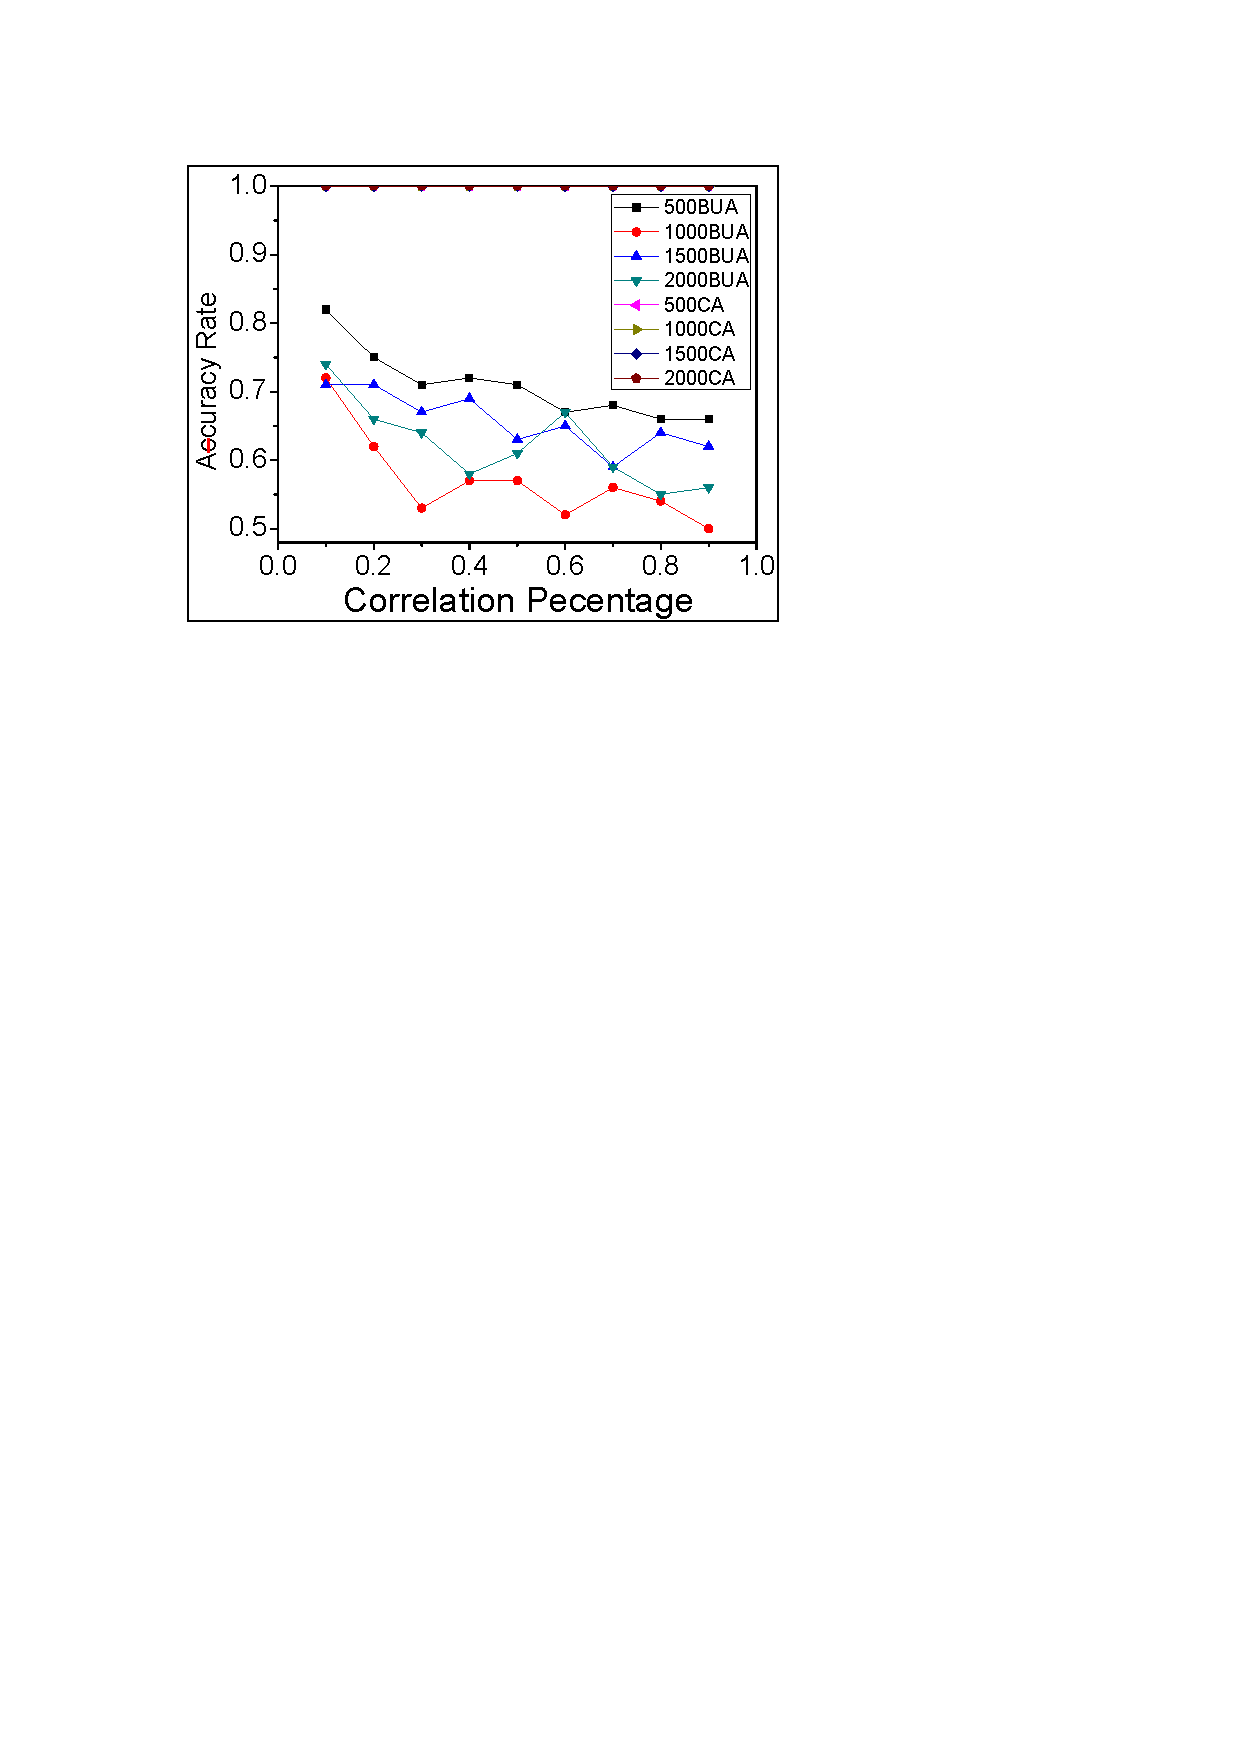
\includegraphics[width=0.48\textwidth]{./FIGs/Experiments/csky_computing/Fig_AccBuaCorr.pdf} \label{fig:fig_AccBuaCorr} }
    \subfigure[CA 与 没有考虑关联的BUA(NCA)] { 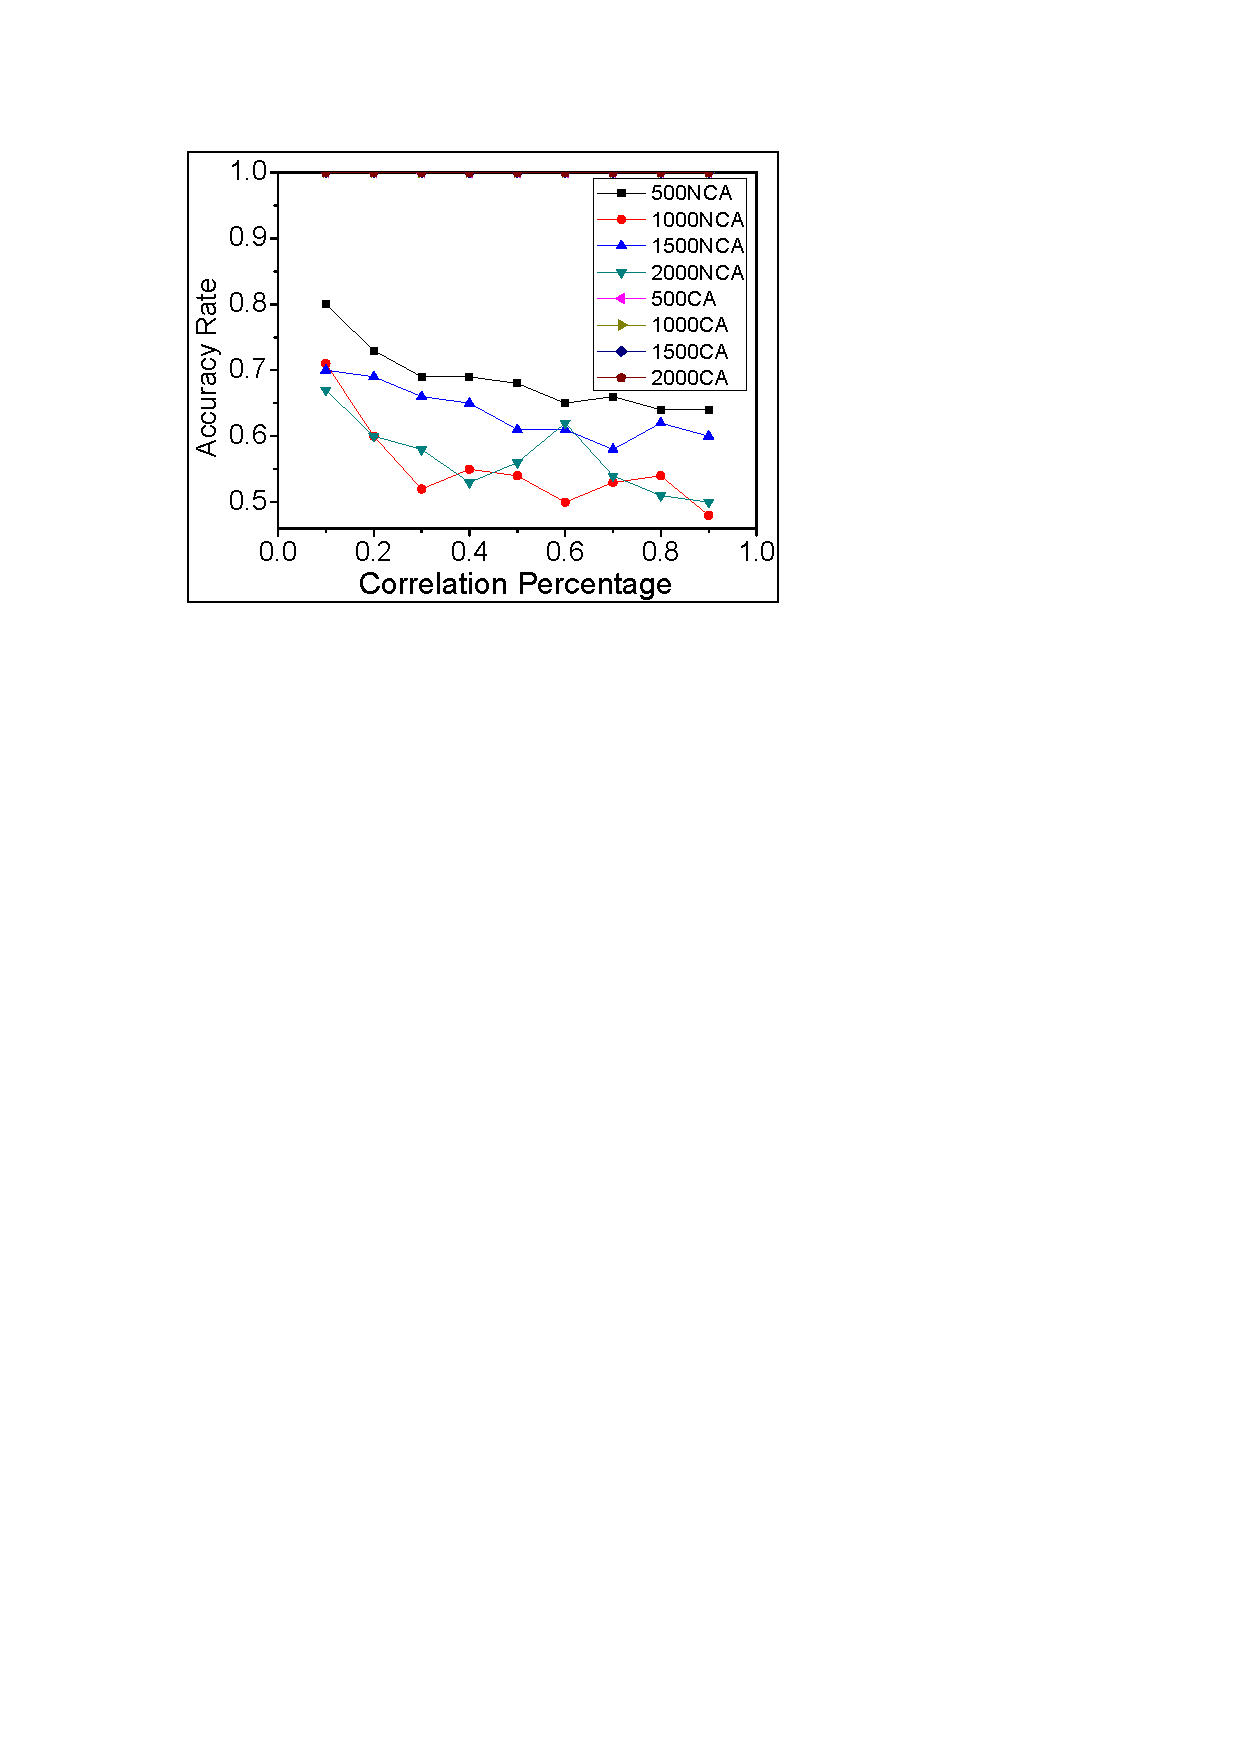
\includegraphics[width=0.48\textwidth]{./FIGs/Experiments/csky_computing/Fig_AccBuaNoCorr.pdf} \label{fig:fig_AccBuaNoCorr} }
    \caption{方法的准确性}
    \label{F:Fig_Exp_Accuracy}
  \end{minipage}%
\end{figure*}


\subsubsection{实验二:验证我们算法是否可以削减候选服务集合大小}

在本节,我们将验证我们的方法是否可以削减候选服务集合的大小。候选服务集合中的服务是服务分解后的结果。我们在本实验中,我们使用的系统生成的数据集,候选服务集合的大小是1000,抽象服务的数量设置为4,QoS~属性数量设置为3。结果如图~\ref{F:Fig_Exp_EffiCand}~所示,我们可以发现使用剪枝算法后,候选服务集合中的服务数量得到了极大的削减。

\begin{figure}[!thb]
    \centering
    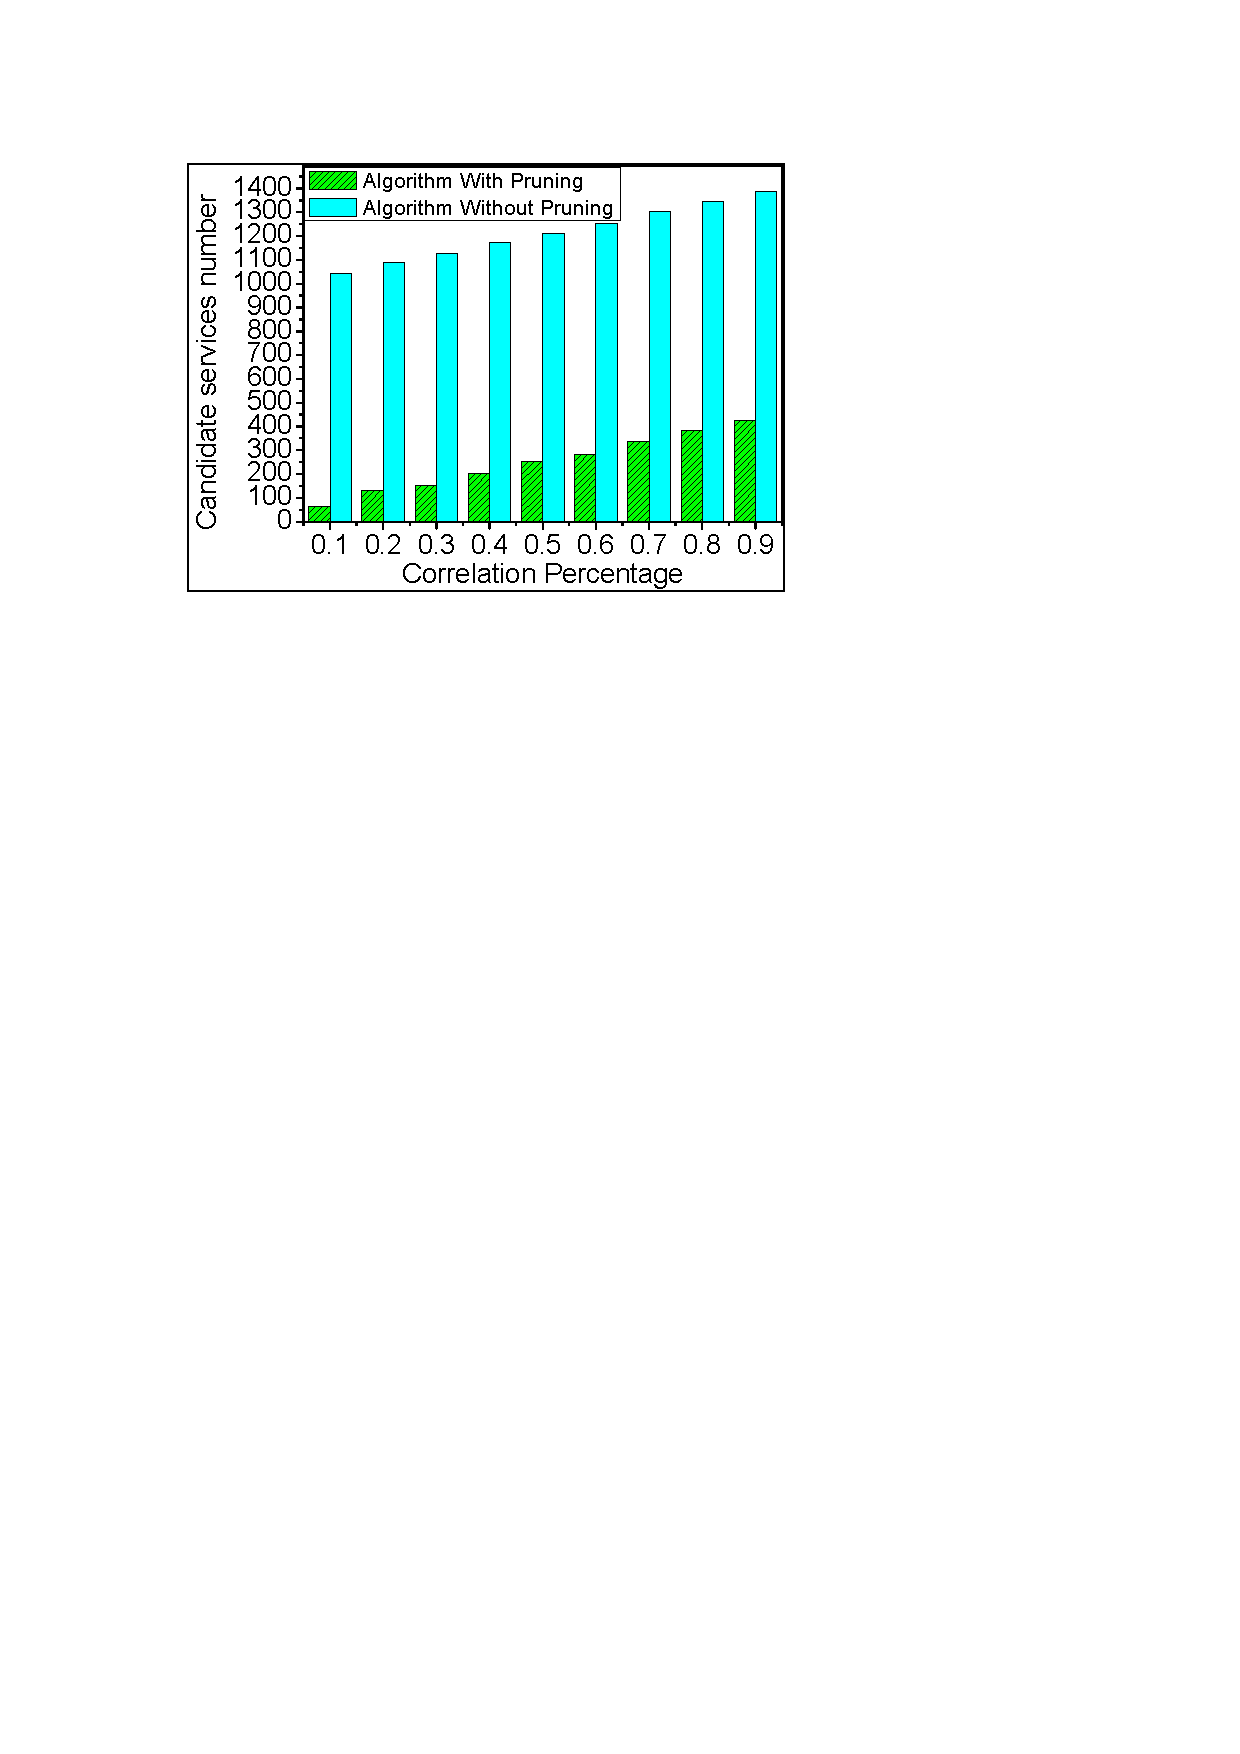
\includegraphics[width=0.48\textwidth]{./FIGs/Experiments/csky_computing/Fig_EffiCand.pdf}
    \caption{剪枝后候选服务集合的大小}
    \label{F:Fig_Exp_EffiCand}
\end{figure}


\subsubsection{实验三:不同关联比重下是否使用剪枝的性能分析}

在本节,我们将比较在不同关联比重下是否使用剪枝的性能,我们分别使用QWS 数据集以及系统生成的数据集,抽象服务数量为4,每个候选服务集合的大小为300,~QoS~属性设置为3个。结果如图~\ref{F:Fig_Exp EffeRtDiffCorr}~所示,我们可以看到无论是在哪一个数据集上,我们算法相比较于不用剪枝的算法都有较大的提高。

\begin{figure*}[!thb]
 \begin{minipage}[b]{1\linewidth} % 如果一行放2 个图,用0.5,如果3 个图,用0.33
    \centering
    \subfigure[算法响应时间(QWS数据集)] { 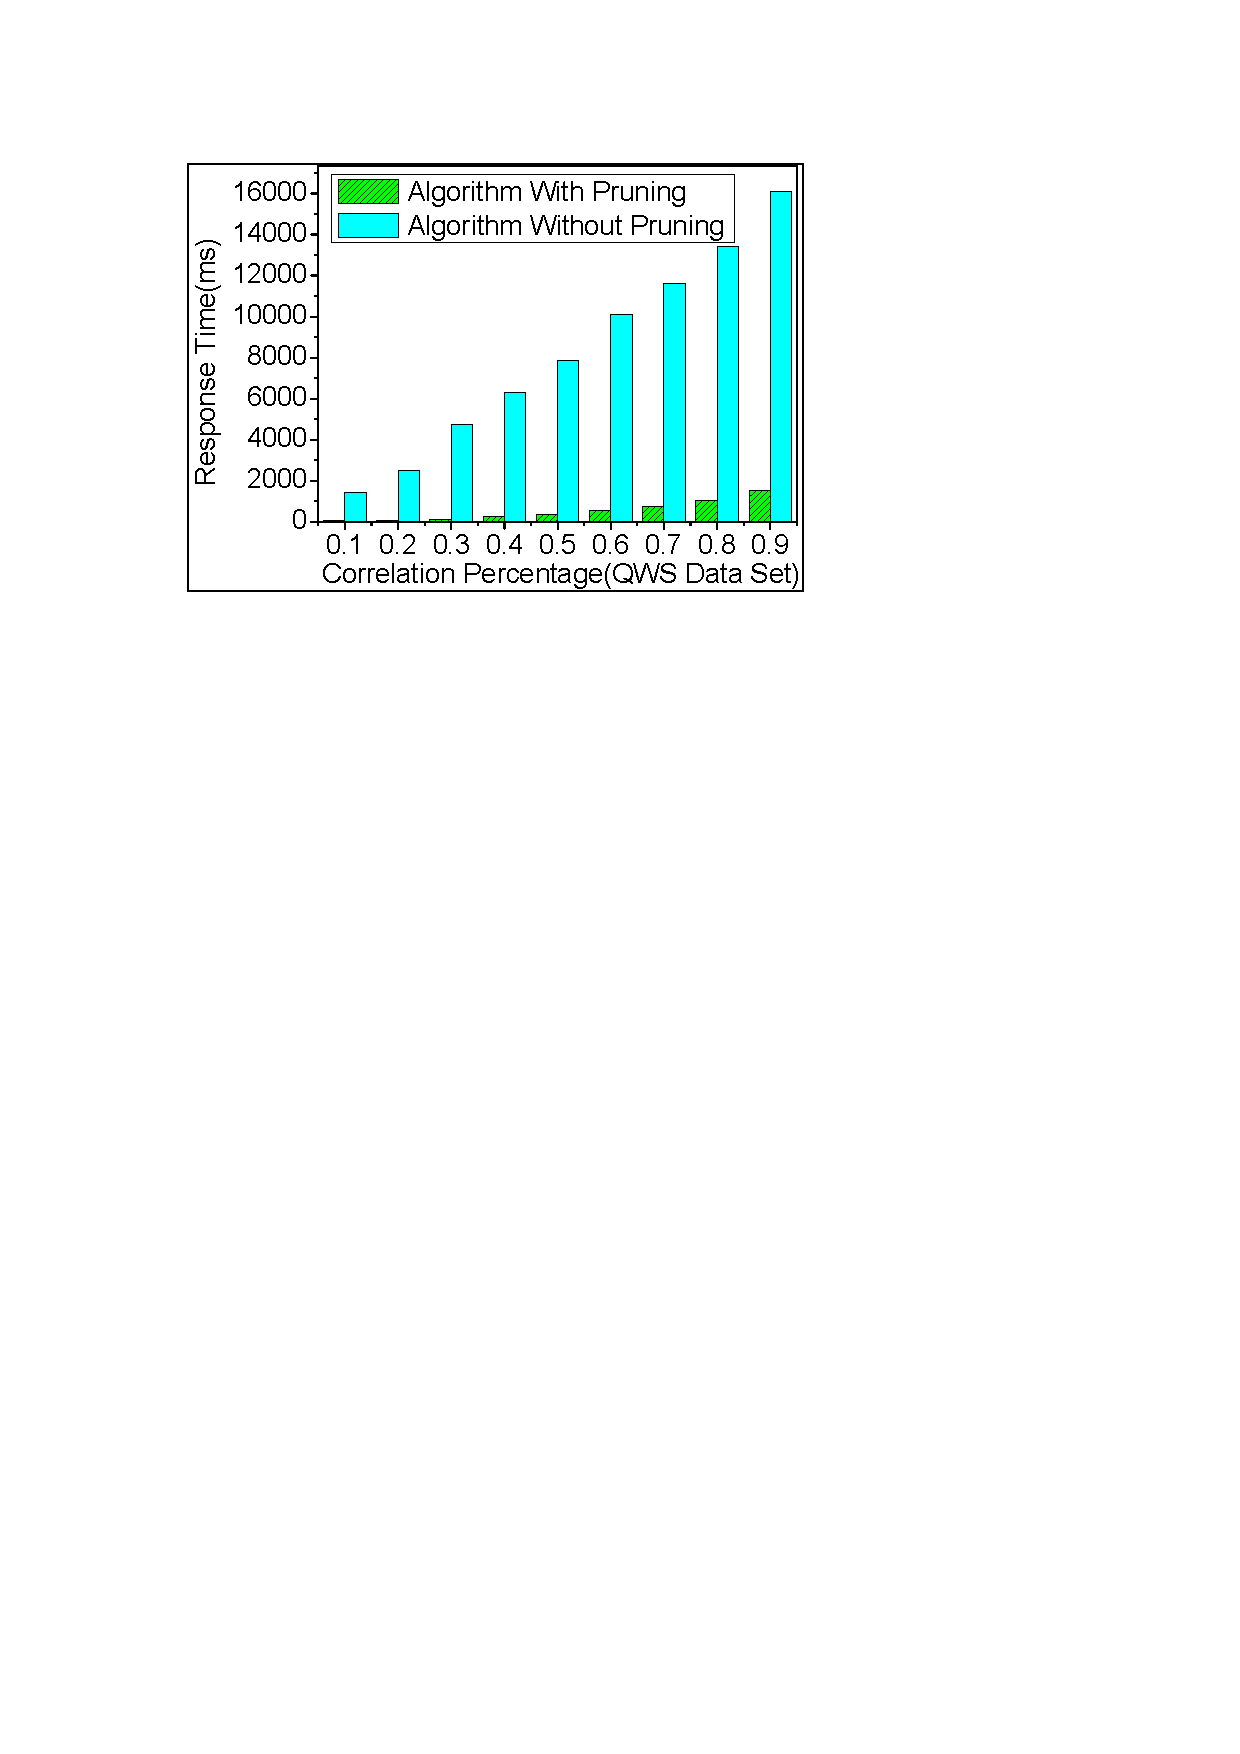
\includegraphics[width=0.47\textwidth]{./FIGs/Experiments/csky_computing/Fig_EffeRtDiffCorrQws.pdf} \label{F:Fig_Exp_EffeRtDiffCorrQws} }
    \hspace{0.05in}
    \subfigure[算法响应时间(系统生成数据集)] { 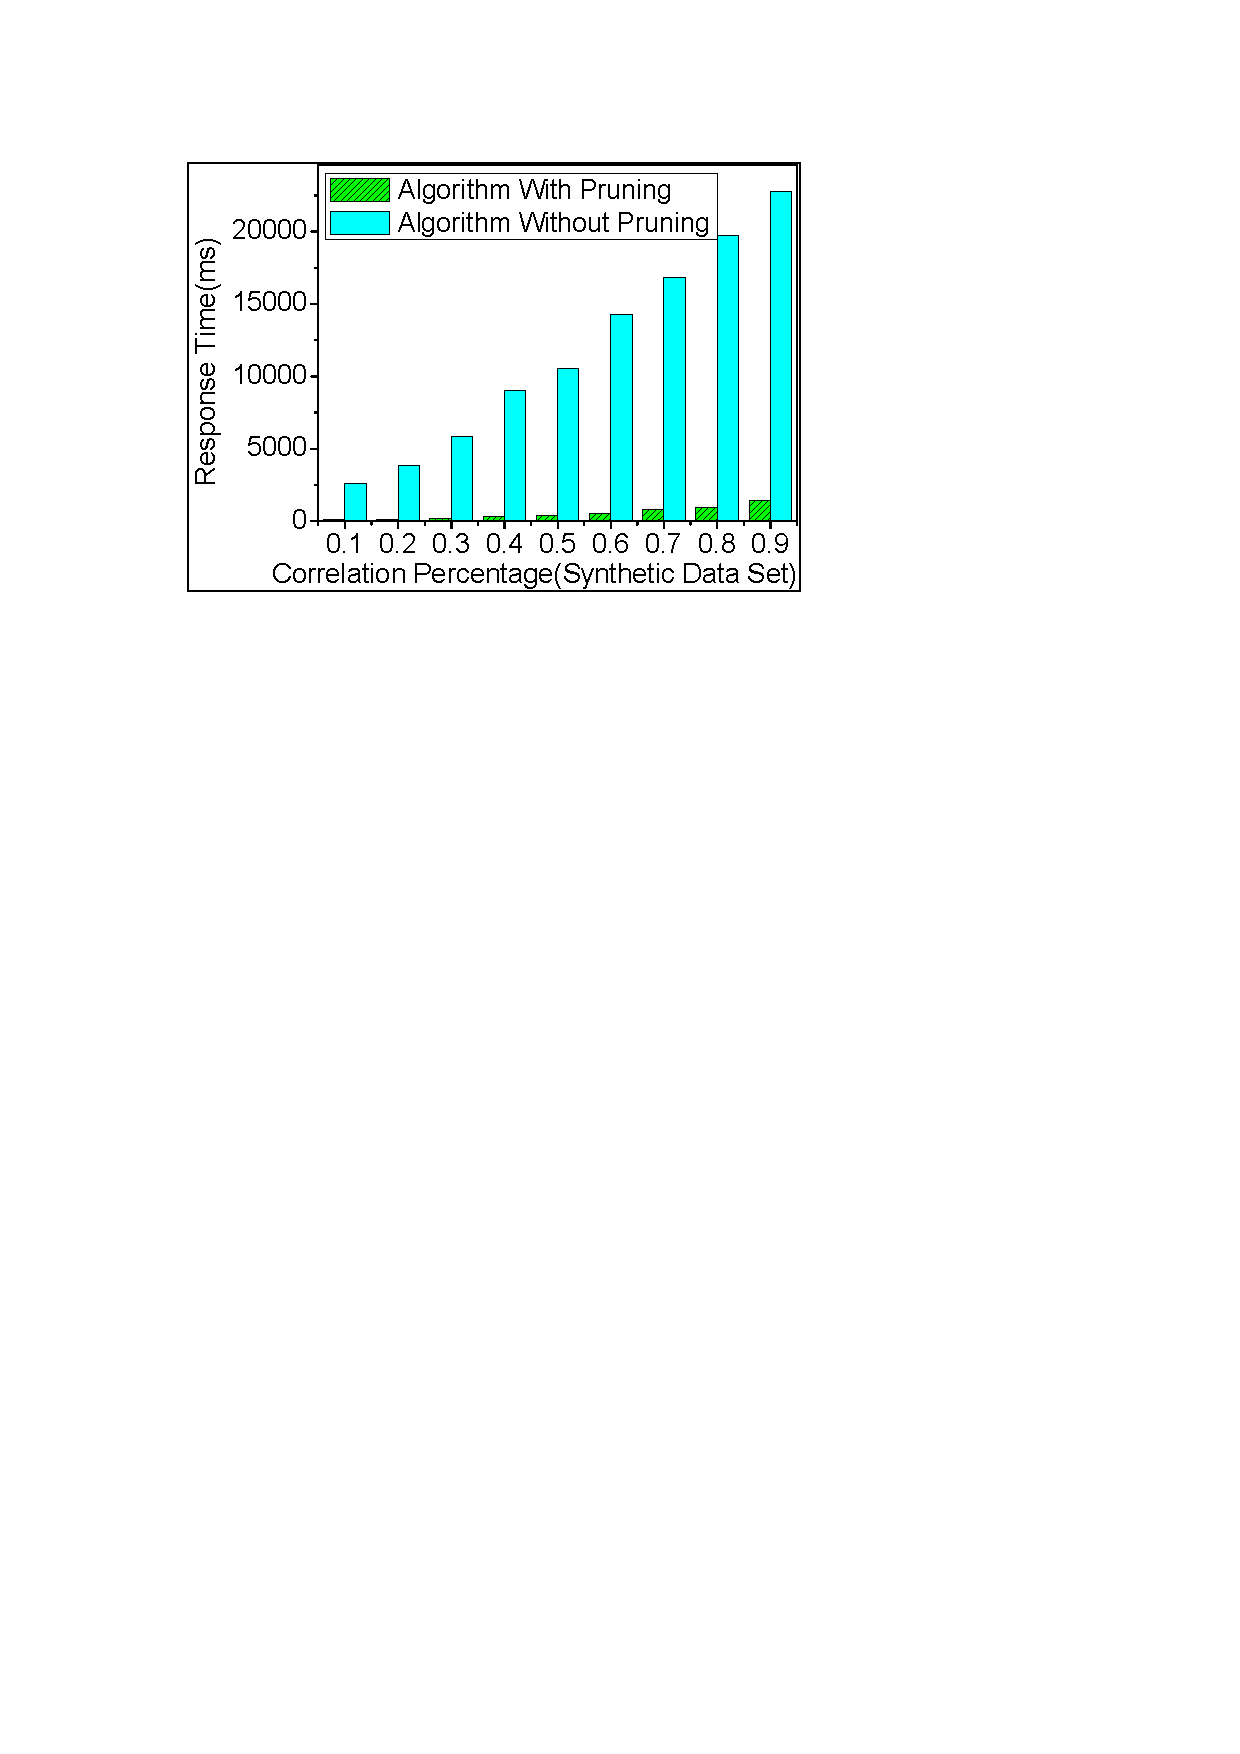
\includegraphics[width=0.47\textwidth]{./FIGs/Experiments/csky_computing/Fig_EffeRtDiffCorrRan.pdf} \label{F:Fig_Exp_EffeRtDiffCorrRan} }
    \caption{不同关联比重下是否使用剪枝的性能分析}
    \label{F:Fig_Exp EffeRtDiffCorr}
  \end{minipage}%
\end{figure*}

\subsection{效率实验}

\subsubsection{实验四:不同QoS属性数量对剪枝算法的影响}

在本节我们将分析不同QoS属性数量对我们算法的影响,我们使用系统生成的数据集,抽象服务的数量设置为4,每个抽象服务对应的候选服务大小设置1000,分别设置~QoS~属性的数量为2,3,4。结果如图~\ref{F:Fig_Exp_EffeCandDiffDimenDiffCorr}~所示,我们可以发现随着属性数量的增大,剪枝的效果也变差。

\begin{figure}[!thb]
    \centering
    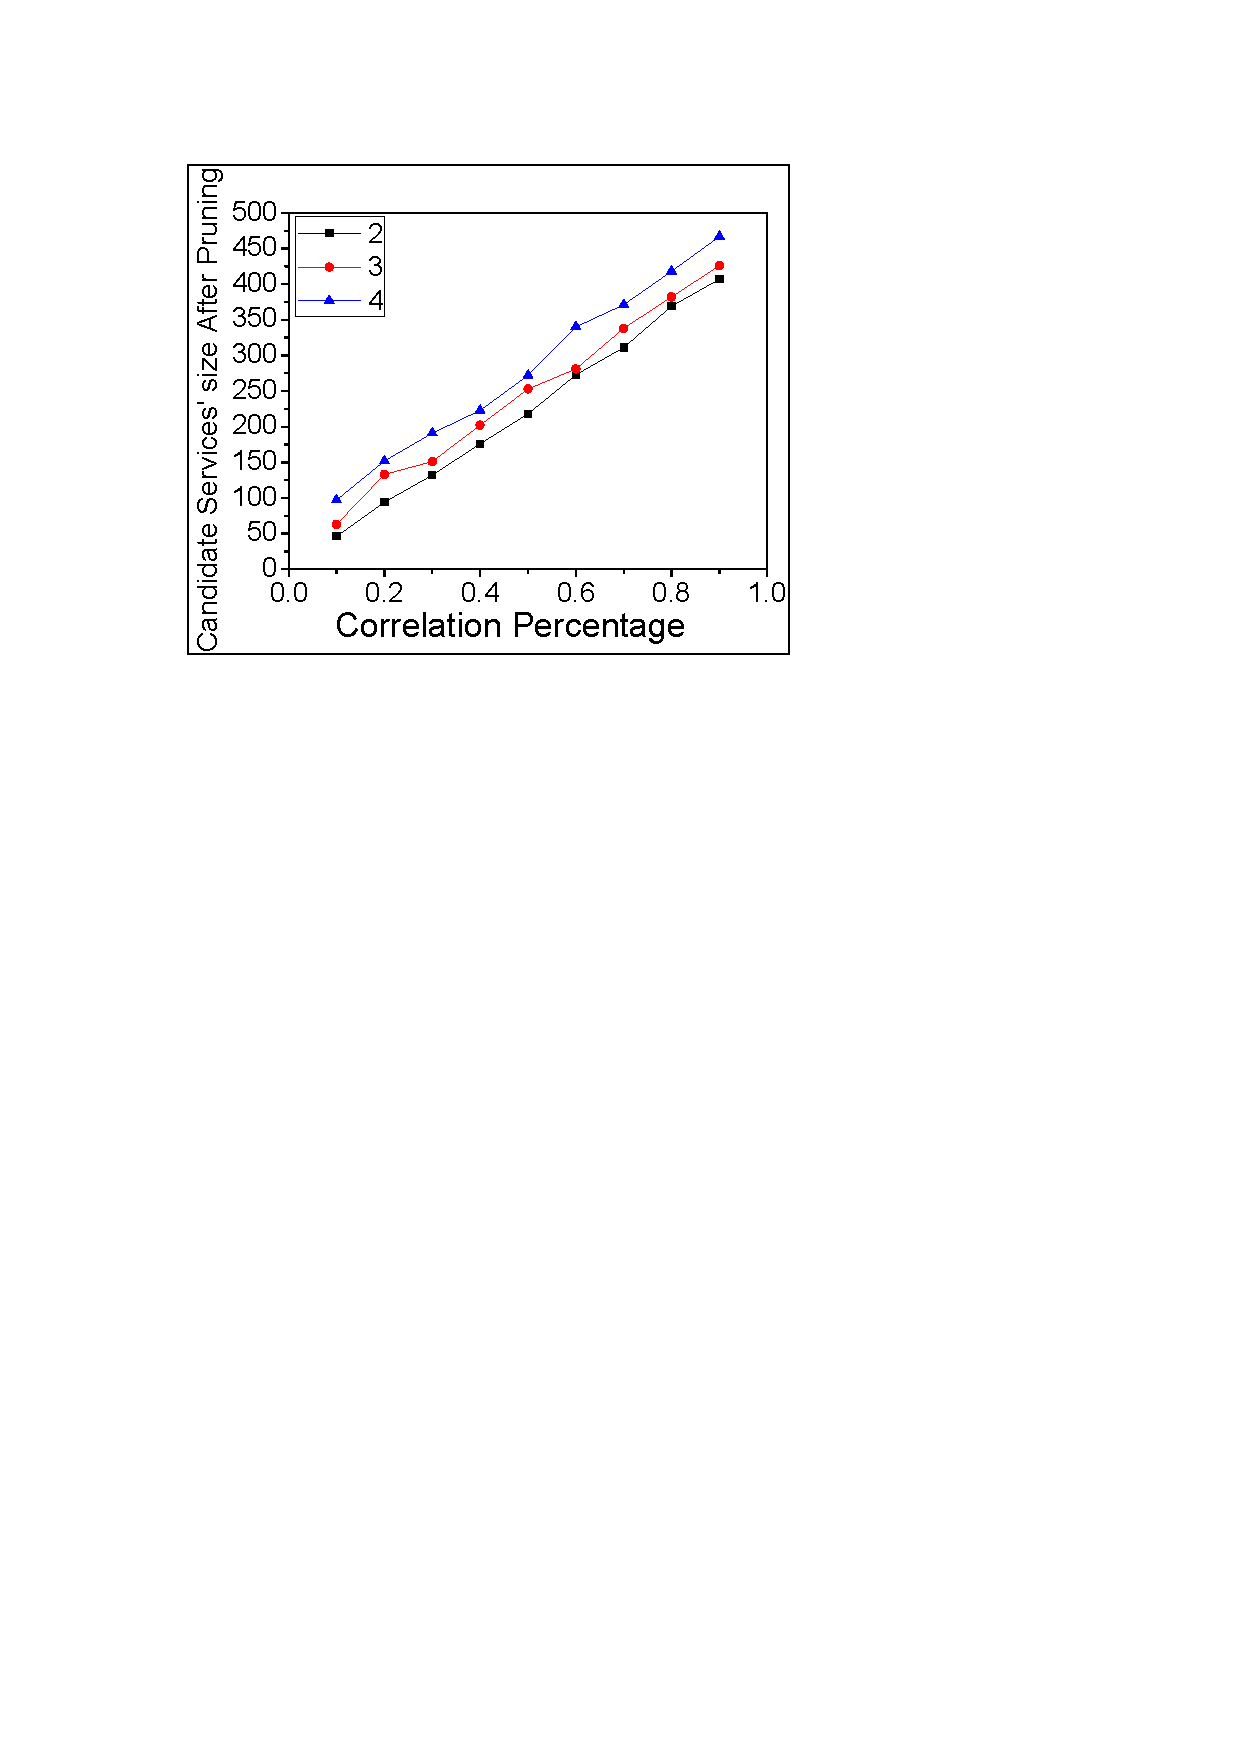
\includegraphics[width=0.48\textwidth]{./FIGs/Experiments/csky_computing/Fig_EffeCandDiffDimenDiffCorr.pdf}
    \caption{不同QoS属性数量对剪枝算法的影响}
    \label{F:Fig_Exp_EffeCandDiffDimenDiffCorr}
\end{figure}


\begin{figure*}[!thb]
 \begin{minipage}[b]{1\linewidth} % 如果一行放2 个图,用0.5,如果3 个图,用0.33
    \centering
    \subfigure[算法2与3的总响应时间] { 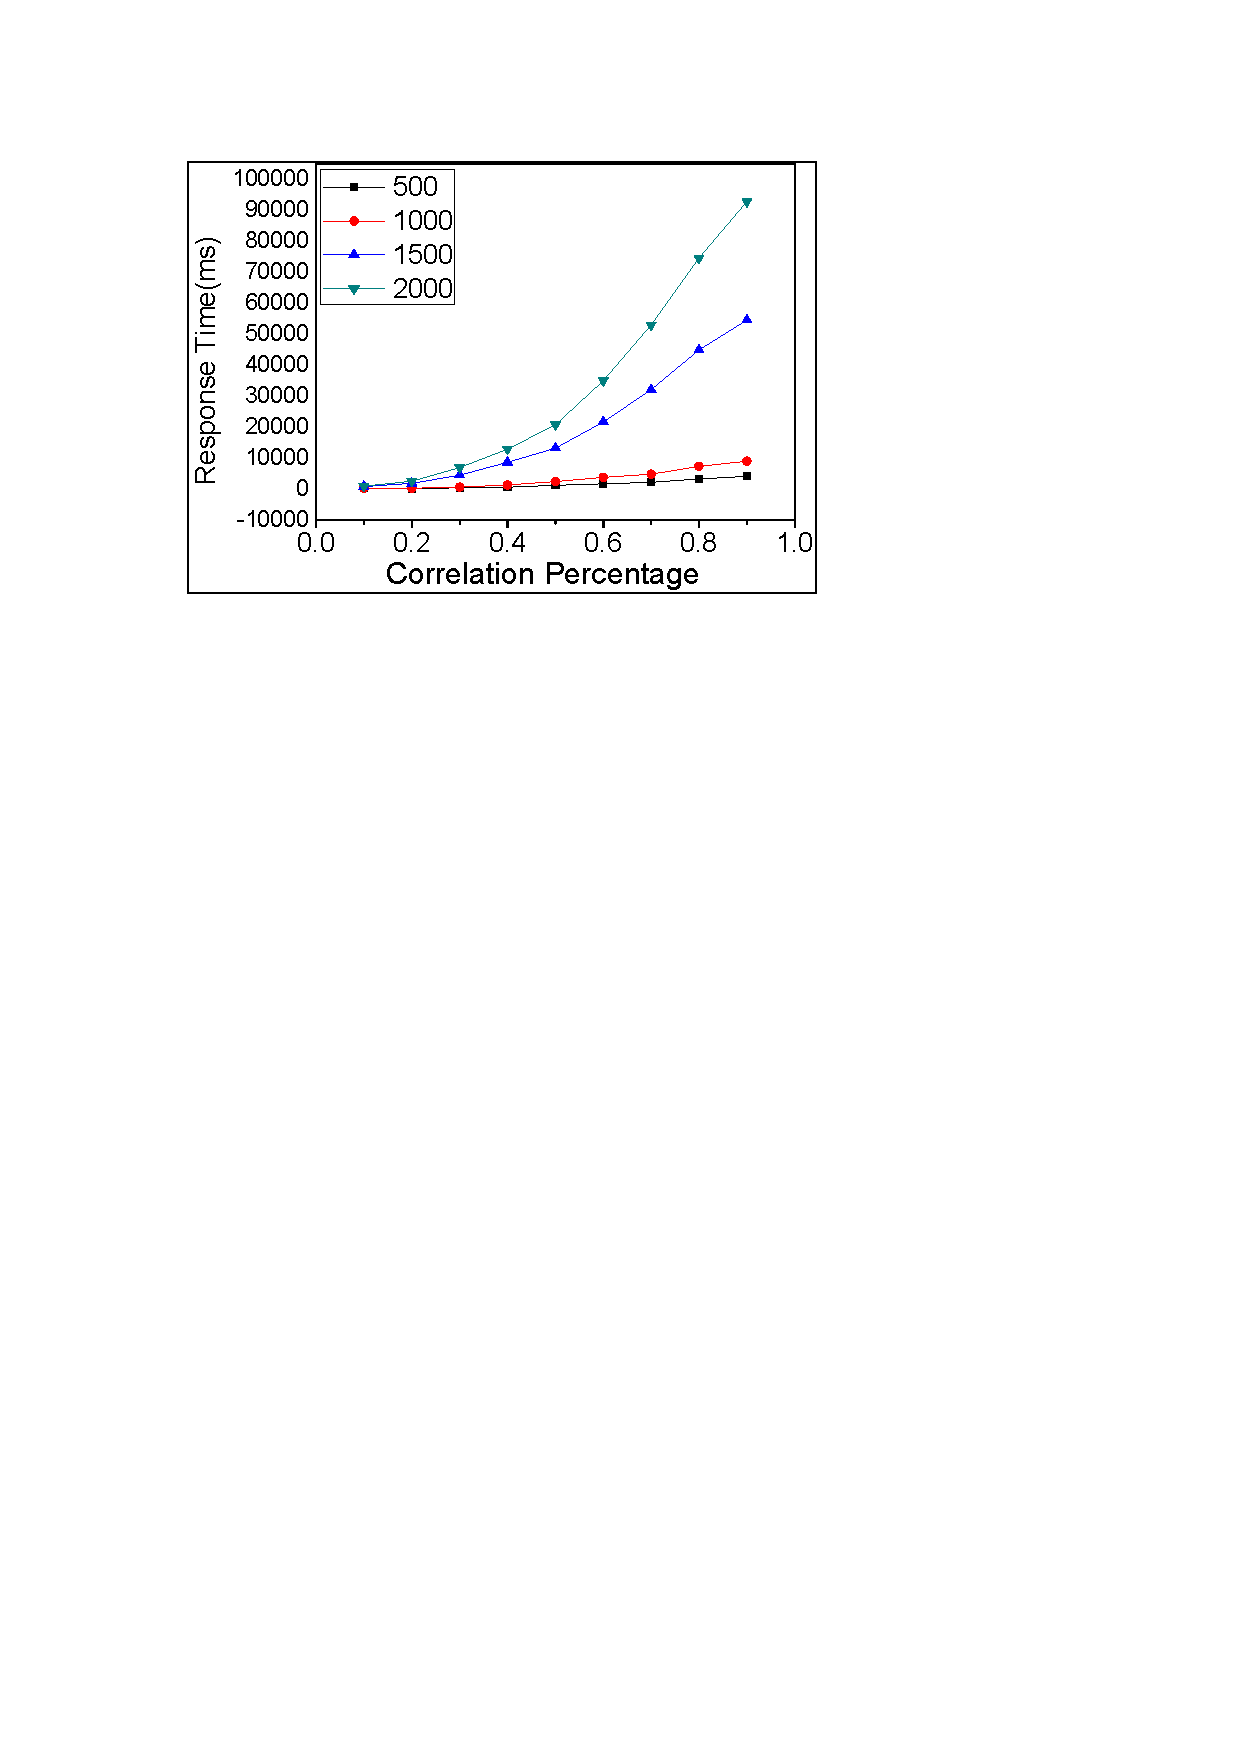
\includegraphics[width=0.47\textwidth,height=2.15in]{./FIGs/Experiments/csky_computing/Fig_EffeRtDiffCanBigAlgo.pdf} \label{F:Fig_Exp_EffeRtDiffCanBigAlgo} }
    \subfigure[算法1的响应时间] { 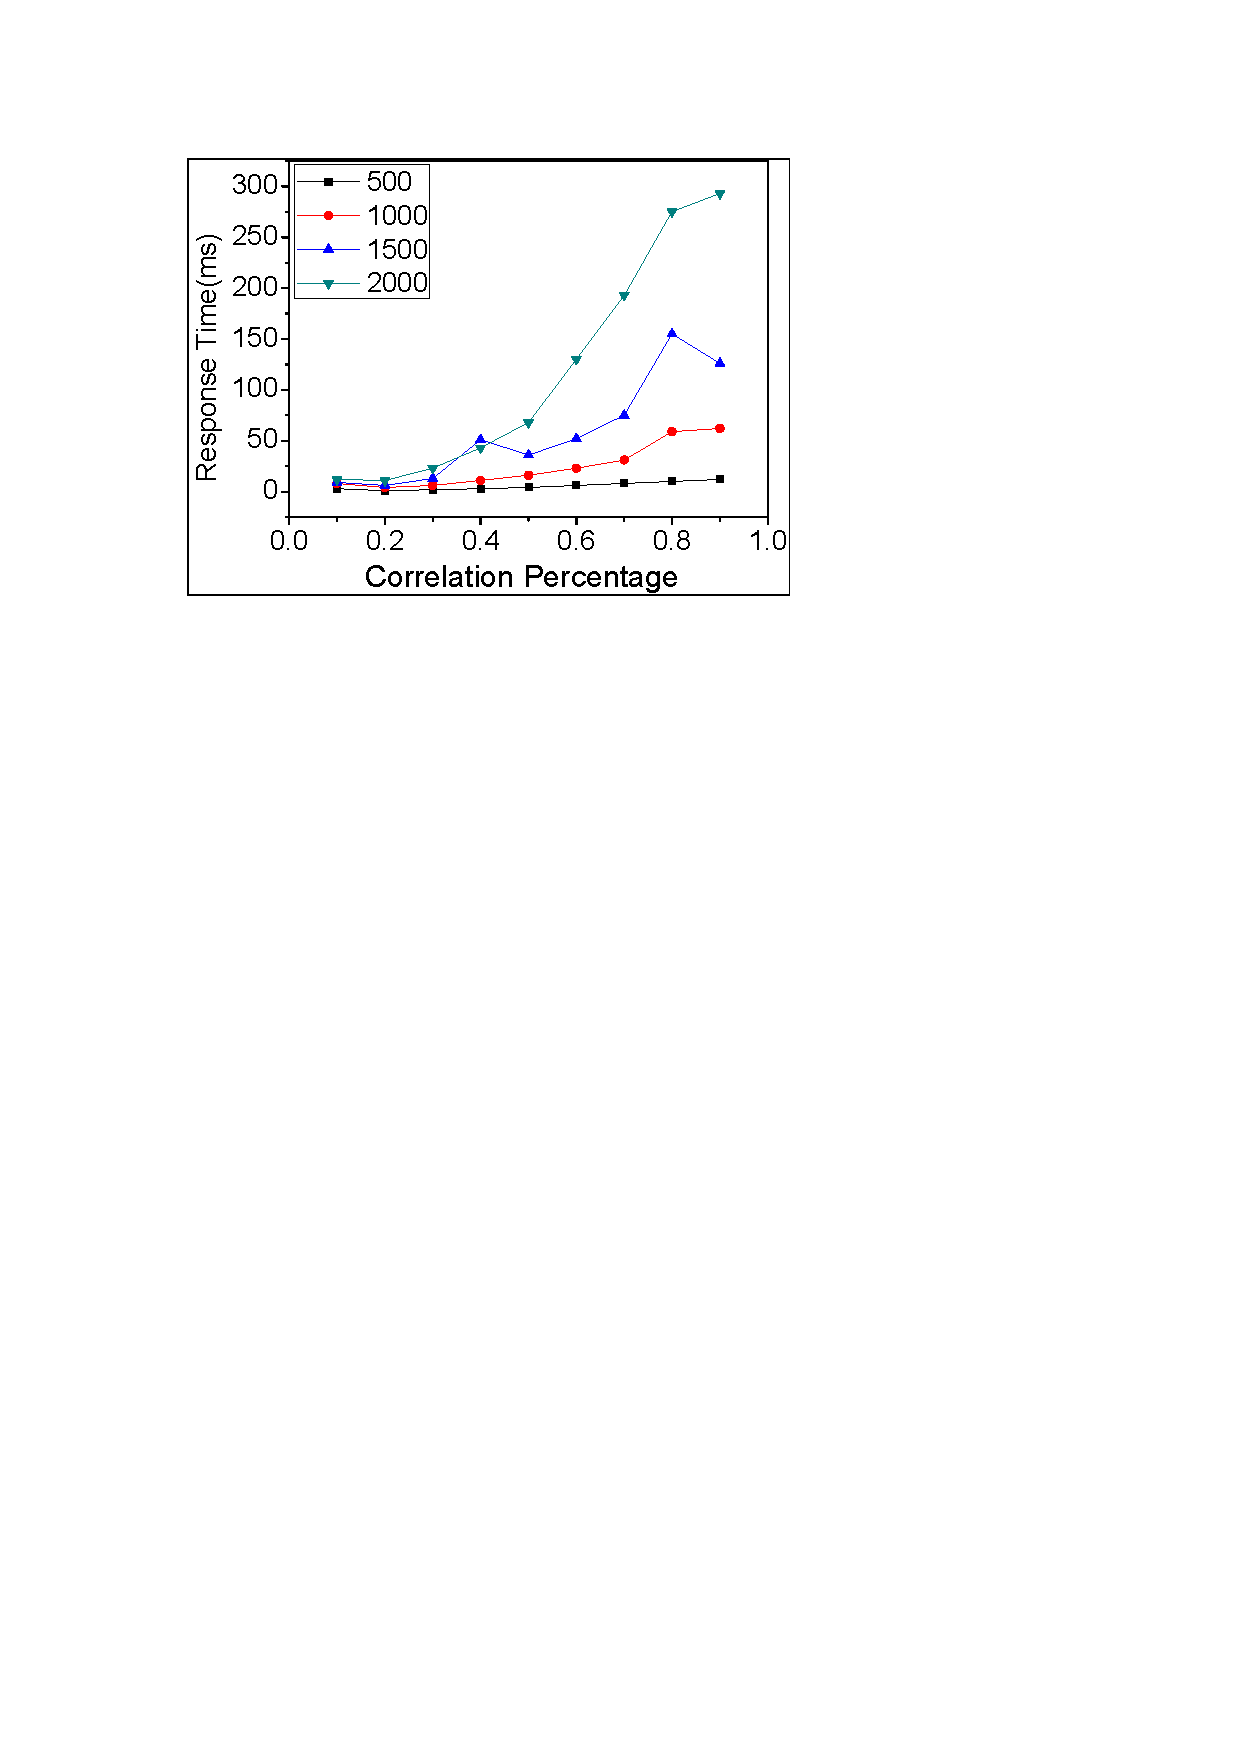
\includegraphics[width=0.47\textwidth, height=2.15in]{./FIGs/Experiments/csky_computing/Fig_EffeRtDiffCanSmallAlgo.pdf} \label{F:Fig_Exp_EffeRtDiffCanSmallAlgo} }
    \caption{不同候选服务集合大小对剪枝算法的影响}
    \label{F:Fig_Exp EffeRtDiffCanDiffAlgo}
  \end{minipage}%
\end{figure*}

\subsubsection{实验五:不同候选服务集合大小对剪枝算法的影响}

在本节我们将分析不同候选服务集合大小对剪枝算法的影响,我们使用系统生成的数据集,抽象服务的数量设置为4,分别设置候选服务大小为500,1000,1500,2000,分别设置~QoS~属性的数量为3。 结果如图~\ref{F:Fig_Exp EffeRtDiffCanDiffAlgo}~ 所示,随着候选服务集合大小增大,剪枝算法的时间也随之增长。



%\subsubsection{实验六:与BUA算法比较}
%
%由于BUA算法只考虑每个候选服务集合中的~Skyline~ 服务,在组合阶段,对中间结果也只考虑~Skyline~子组合服务,因此它的效率一定要比我们考虑~QoS~ 关联的情况要高,这是可以理解也是可以接受的。我们使用系统生成的数据集,抽象服务的数量设置为4,分别设置候选服务大小为500,分别设置~QoS~属性的数量为3,结果如图~\ref{F:Fig_Exp_EffeRtBua}~所示。
%
%\begin{figure}[!thb]
%    \centering
%    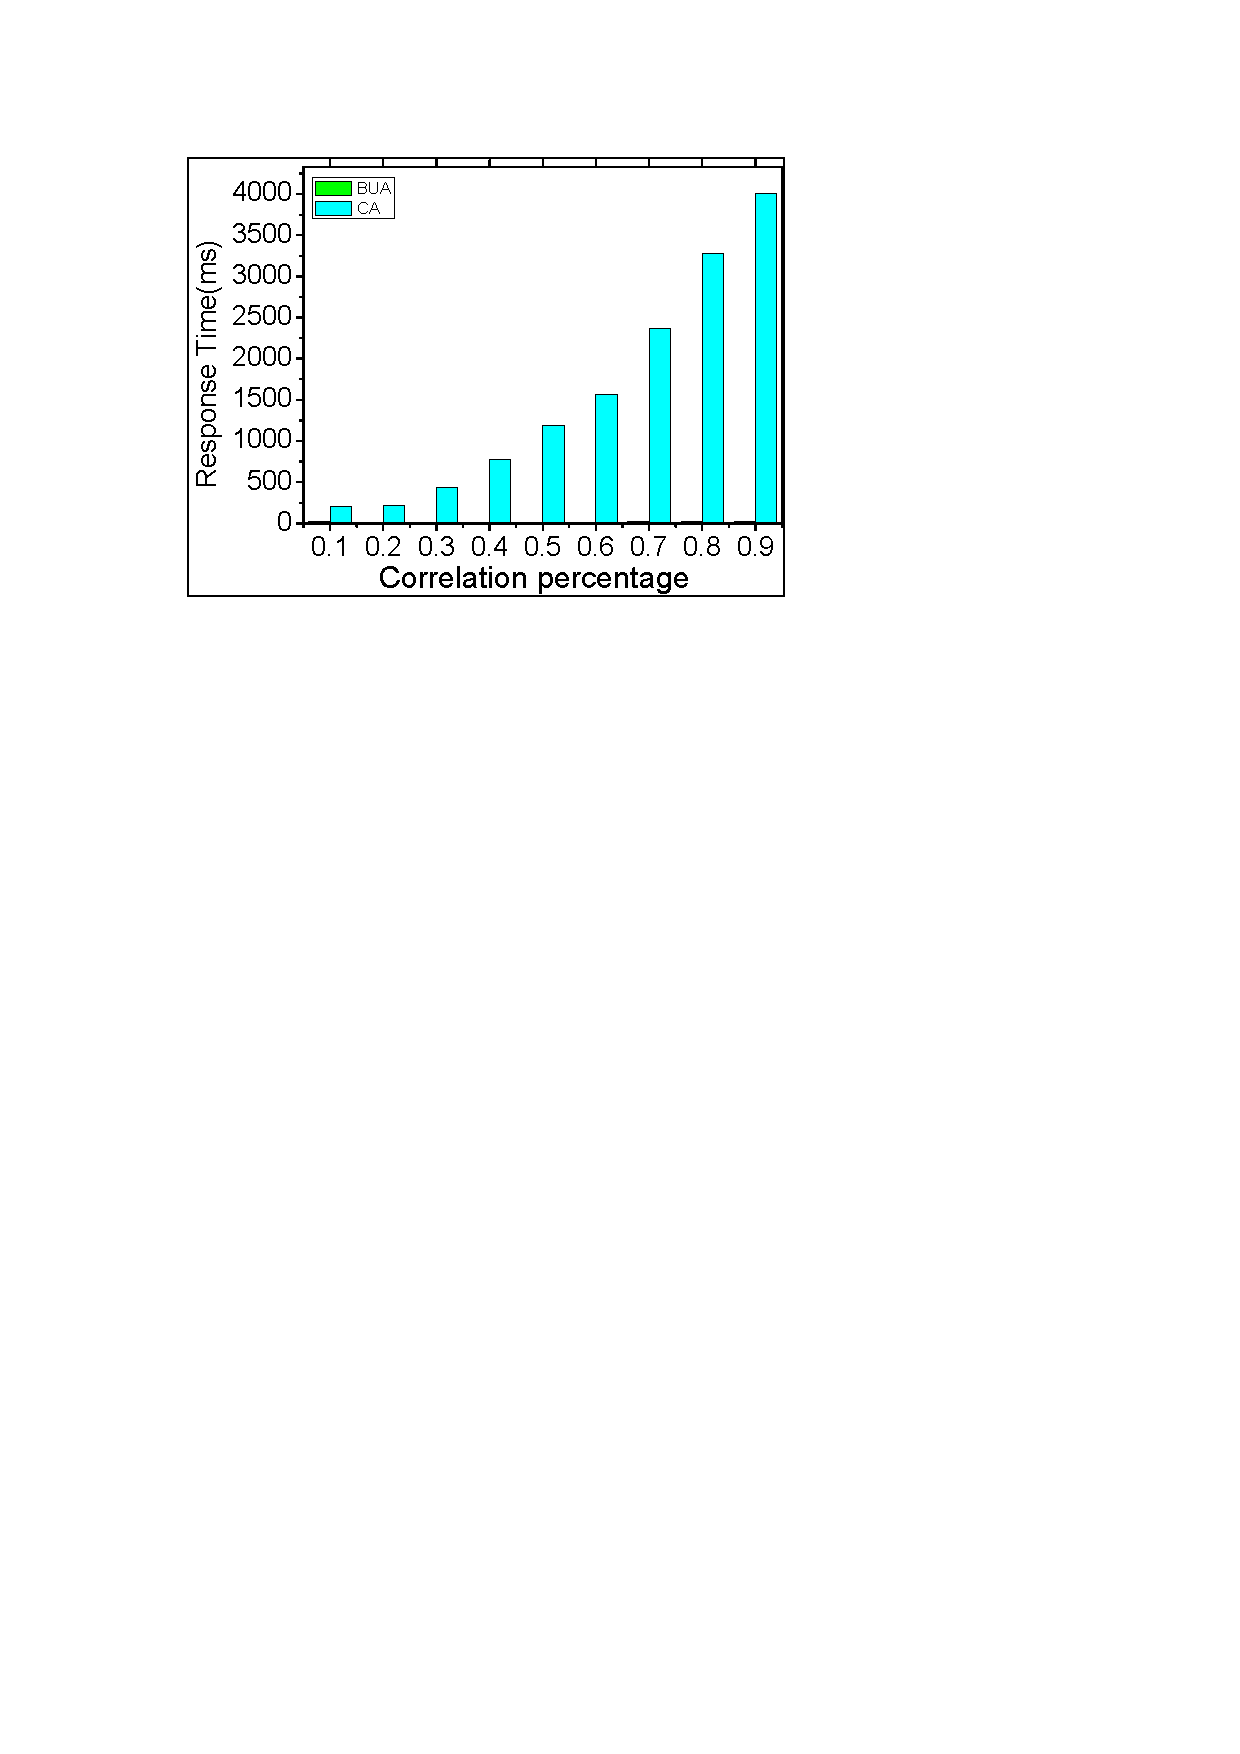
\includegraphics[width=0.48\textwidth]{./FIGs/Experiments/csky_computing/Fig_EffeRtBua.pdf}
%    \caption{与BUA算法比较}
%    \label{F:Fig_Exp_EffeRtBua}
%\end{figure}

\section{本章小结}

我们在本章定义了在存在~QoS~关联的场景下计算组合服务~Skyline~的问题,并给提出一种支持QoS关联的组合服务~Skyline~计算方法。我们提出了一系列剪枝规则来提高我们方法的效率。最后,我们通过一些列实验来分析我们方法的有效性以及效率。